\documentclass[11pt]{article}

    \usepackage[breakable]{tcolorbox}
    \usepackage{parskip} % Stop auto-indenting (to mimic markdown behaviour)
    

    % Basic figure setup, for now with no caption control since it's done
    % automatically by Pandoc (which extracts ![](path) syntax from Markdown).
    \usepackage{graphicx}
    % Maintain compatibility with old templates. Remove in nbconvert 6.0
    \let\Oldincludegraphics\includegraphics
    % Ensure that by default, figures have no caption (until we provide a
    % proper Figure object with a Caption API and a way to capture that
    % in the conversion process - todo).
    \usepackage{caption}
    % \DeclareCaptionFormat{nocaption}{}`
    % \captionsetup{format=nocaption,aboveskip=0pt,belowskip=0pt}

    \usepackage{float}
    \floatplacement{figure}{H} % forces figures to be placed at the correct location
    \usepackage{xcolor} % Allow colors to be defined
    \usepackage{enumerate} % Needed for markdown enumerations to work
    \usepackage{geometry} % Used to adjust the document margins
    \usepackage{amsmath} % Equations
    \usepackage{amssymb} % Equations
    \usepackage{textcomp} % defines textquotesingle
    % Hack from http://tex.stackexchange.com/a/47451/13684:
    \AtBeginDocument{%
        \def\PYZsq{\textquotesingle}% Upright quotes in Pygmentized code
    }
    \usepackage{upquote} % Upright quotes for verbatim code
    \usepackage{eurosym} % defines \euro

    \usepackage{iftex}
    \ifPDFTeX
        \usepackage[T1]{fontenc}
        \IfFileExists{alphabeta.sty}{
              \usepackage{alphabeta}
          }{
              \usepackage[mathletters]{ucs}
              \usepackage[utf8x]{inputenc}
          }
    \else
        \usepackage{fontspec}
        \usepackage{unicode-math}
    \fi

    \usepackage{fancyvrb} % verbatim replacement that allows latex
    \usepackage{grffile} % extends the file name processing of package graphics 
                         % to support a larger range
    \makeatletter % fix for old versions of grffile with XeLaTeX
    \@ifpackagelater{grffile}{2019/11/01}
    {
      % Do nothing on new versions
    }
    {
      \def\Gread@@xetex#1{%
        \IfFileExists{"\Gin@base".bb}%
        {\Gread@eps{\Gin@base.bb}}%
        {\Gread@@xetex@aux#1}%
      }
    }
    \makeatother
    \usepackage[Export]{adjustbox} % Used to constrain images to a maximum size
    \adjustboxset{max size={0.9\linewidth}{0.9\paperheight}}

    % The hyperref package gives us a pdf with properly built
    % internal navigation ('pdf bookmarks' for the table of contents,
    % internal cross-reference links, web links for URLs, etc.)
    \usepackage{hyperref}
    % The default LaTeX title has an obnoxious amount of whitespace. By default,
    % titling removes some of it. It also provides customization options.
    \usepackage{titling}
    \usepackage{longtable} % longtable support required by pandoc >1.10
    \usepackage{booktabs}  % table support for pandoc > 1.12.2
    \usepackage{array}     % table support for pandoc >= 2.11.3
    \usepackage{calc}      % table minipage width calculation for pandoc >= 2.11.1
    \usepackage[inline]{enumitem} % IRkernel/repr support (it uses the enumerate* environment)
    \usepackage[normalem]{ulem} % ulem is needed to support strikethroughs (\sout)
                                % normalem makes italics be italics, not underlines
    \usepackage{mathrsfs}
    \usepackage{hyperref}

    
    % Colors for the hyperref package
    \definecolor{urlcolor}{rgb}{0,.145,.698}
    \definecolor{linkcolor}{rgb}{.71,0.21,0.01}
    \definecolor{citecolor}{rgb}{.12,.54,.11}

    % ANSI colors
    \definecolor{ansi-black}{HTML}{3E424D}
    \definecolor{ansi-black-intense}{HTML}{282C36}
    \definecolor{ansi-red}{HTML}{E75C58}
    \definecolor{ansi-red-intense}{HTML}{B22B31}
    \definecolor{ansi-green}{HTML}{00A250}
    \definecolor{ansi-green-intense}{HTML}{007427}
    \definecolor{ansi-yellow}{HTML}{DDB62B}
    \definecolor{ansi-yellow-intense}{HTML}{B27D12}
    \definecolor{ansi-blue}{HTML}{208FFB}
    \definecolor{ansi-blue-intense}{HTML}{0065CA}
    \definecolor{ansi-magenta}{HTML}{D160C4}
    \definecolor{ansi-magenta-intense}{HTML}{A03196}
    \definecolor{ansi-cyan}{HTML}{60C6C8}
    \definecolor{ansi-cyan-intense}{HTML}{258F8F}
    \definecolor{ansi-white}{HTML}{C5C1B4}
    \definecolor{ansi-white-intense}{HTML}{A1A6B2}
    \definecolor{ansi-default-inverse-fg}{HTML}{FFFFFF}
    \definecolor{ansi-default-inverse-bg}{HTML}{000000}

    % common color for the border for error outputs.
    \definecolor{outerrorbackground}{HTML}{FFDFDF}

    % commands and environments needed by pandoc snippets
    % extracted from the output of `pandoc -s`
    \providecommand{\tightlist}{%
      \setlength{\itemsep}{0pt}\setlength{\parskip}{0pt}}
    \DefineVerbatimEnvironment{Highlighting}{Verbatim}{commandchars=\\\{\}}
    % Add ',fontsize=\small' for more characters per line
    \newenvironment{Shaded}{}{}
    \newcommand{\KeywordTok}[1]{\textcolor[rgb]{0.00,0.44,0.13}{\textbf{{#1}}}}
    \newcommand{\DataTypeTok}[1]{\textcolor[rgb]{0.56,0.13,0.00}{{#1}}}
    \newcommand{\DecValTok}[1]{\textcolor[rgb]{0.25,0.63,0.44}{{#1}}}
    \newcommand{\BaseNTok}[1]{\textcolor[rgb]{0.25,0.63,0.44}{{#1}}}
    \newcommand{\FloatTok}[1]{\textcolor[rgb]{0.25,0.63,0.44}{{#1}}}
    \newcommand{\CharTok}[1]{\textcolor[rgb]{0.25,0.44,0.63}{{#1}}}
    \newcommand{\StringTok}[1]{\textcolor[rgb]{0.25,0.44,0.63}{{#1}}}
    \newcommand{\CommentTok}[1]{\textcolor[rgb]{0.38,0.63,0.69}{\textit{{#1}}}}
    \newcommand{\OtherTok}[1]{\textcolor[rgb]{0.00,0.44,0.13}{{#1}}}
    \newcommand{\AlertTok}[1]{\textcolor[rgb]{1.00,0.00,0.00}{\textbf{{#1}}}}
    \newcommand{\FunctionTok}[1]{\textcolor[rgb]{0.02,0.16,0.49}{{#1}}}
    \newcommand{\RegionMarkerTok}[1]{{#1}}
    \newcommand{\ErrorTok}[1]{\textcolor[rgb]{1.00,0.00,0.00}{\textbf{{#1}}}}
    \newcommand{\NormalTok}[1]{{#1}}
    
    % Additional commands for more recent versions of Pandoc
    \newcommand{\ConstantTok}[1]{\textcolor[rgb]{0.53,0.00,0.00}{{#1}}}
    \newcommand{\SpecialCharTok}[1]{\textcolor[rgb]{0.25,0.44,0.63}{{#1}}}
    \newcommand{\VerbatimStringTok}[1]{\textcolor[rgb]{0.25,0.44,0.63}{{#1}}}
    \newcommand{\SpecialStringTok}[1]{\textcolor[rgb]{0.73,0.40,0.53}{{#1}}}
    \newcommand{\ImportTok}[1]{{#1}}
    \newcommand{\DocumentationTok}[1]{\textcolor[rgb]{0.73,0.13,0.13}{\textit{{#1}}}}
    \newcommand{\AnnotationTok}[1]{\textcolor[rgb]{0.38,0.63,0.69}{\textbf{\textit{{#1}}}}}
    \newcommand{\CommentVarTok}[1]{\textcolor[rgb]{0.38,0.63,0.69}{\textbf{\textit{{#1}}}}}
    \newcommand{\VariableTok}[1]{\textcolor[rgb]{0.10,0.09,0.49}{{#1}}}
    \newcommand{\ControlFlowTok}[1]{\textcolor[rgb]{0.00,0.44,0.13}{\textbf{{#1}}}}
    \newcommand{\OperatorTok}[1]{\textcolor[rgb]{0.40,0.40,0.40}{{#1}}}
    \newcommand{\BuiltInTok}[1]{{#1}}
    \newcommand{\ExtensionTok}[1]{{#1}}
    \newcommand{\PreprocessorTok}[1]{\textcolor[rgb]{0.74,0.48,0.00}{{#1}}}
    \newcommand{\AttributeTok}[1]{\textcolor[rgb]{0.49,0.56,0.16}{{#1}}}
    \newcommand{\InformationTok}[1]{\textcolor[rgb]{0.38,0.63,0.69}{\textbf{\textit{{#1}}}}}
    \newcommand{\WarningTok}[1]{\textcolor[rgb]{0.38,0.63,0.69}{\textbf{\textit{{#1}}}}}
    
    
    % Define a nice break command that doesn't care if a line doesn't already
    % exist.
    \def\br{\hspace*{\fill} \\* }
    % Math Jax compatibility definitions
    \def\gt{>}
    \def\lt{<}
    \let\Oldtex\TeX
    \let\Oldlatex\LaTeX
    \renewcommand{\TeX}{\textrm{\Oldtex}}
    \renewcommand{\LaTeX}{\textrm{\Oldlatex}}
    % Document parameters
    % Document title
    \title{Airline Satisfaction - Executive Summary}
    \author{
        Dániel Bence Papp
    }
    
    \usepackage{siunitx}
    
% Pygments definitions
\makeatletter
\def\PY@reset{\let\PY@it=\relax \let\PY@bf=\relax%
    \let\PY@ul=\relax \let\PY@tc=\relax%
    \let\PY@bc=\relax \let\PY@ff=\relax}
\def\PY@tok#1{\csname PY@tok@#1\endcsname}
\def\PY@toks#1+{\ifx\relax#1\empty\else%
    \PY@tok{#1}\expandafter\PY@toks\fi}
\def\PY@do#1{\PY@bc{\PY@tc{\PY@ul{%
    \PY@it{\PY@bf{\PY@ff{#1}}}}}}}
\def\PY#1#2{\PY@reset\PY@toks#1+\relax+\PY@do{#2}}

\@namedef{PY@tok@w}{\def\PY@tc##1{\textcolor[rgb]{0.73,0.73,0.73}{##1}}}
\@namedef{PY@tok@c}{\let\PY@it=\textit\def\PY@tc##1{\textcolor[rgb]{0.24,0.48,0.48}{##1}}}
\@namedef{PY@tok@cp}{\def\PY@tc##1{\textcolor[rgb]{0.61,0.40,0.00}{##1}}}
\@namedef{PY@tok@k}{\let\PY@bf=\textbf\def\PY@tc##1{\textcolor[rgb]{0.00,0.50,0.00}{##1}}}
\@namedef{PY@tok@kp}{\def\PY@tc##1{\textcolor[rgb]{0.00,0.50,0.00}{##1}}}
\@namedef{PY@tok@kt}{\def\PY@tc##1{\textcolor[rgb]{0.69,0.00,0.25}{##1}}}
\@namedef{PY@tok@o}{\def\PY@tc##1{\textcolor[rgb]{0.40,0.40,0.40}{##1}}}
\@namedef{PY@tok@ow}{\let\PY@bf=\textbf\def\PY@tc##1{\textcolor[rgb]{0.67,0.13,1.00}{##1}}}
\@namedef{PY@tok@nb}{\def\PY@tc##1{\textcolor[rgb]{0.00,0.50,0.00}{##1}}}
\@namedef{PY@tok@nf}{\def\PY@tc##1{\textcolor[rgb]{0.00,0.00,1.00}{##1}}}
\@namedef{PY@tok@nc}{\let\PY@bf=\textbf\def\PY@tc##1{\textcolor[rgb]{0.00,0.00,1.00}{##1}}}
\@namedef{PY@tok@nn}{\let\PY@bf=\textbf\def\PY@tc##1{\textcolor[rgb]{0.00,0.00,1.00}{##1}}}
\@namedef{PY@tok@ne}{\let\PY@bf=\textbf\def\PY@tc##1{\textcolor[rgb]{0.80,0.25,0.22}{##1}}}
\@namedef{PY@tok@nv}{\def\PY@tc##1{\textcolor[rgb]{0.10,0.09,0.49}{##1}}}
\@namedef{PY@tok@no}{\def\PY@tc##1{\textcolor[rgb]{0.53,0.00,0.00}{##1}}}
\@namedef{PY@tok@nl}{\def\PY@tc##1{\textcolor[rgb]{0.46,0.46,0.00}{##1}}}
\@namedef{PY@tok@ni}{\let\PY@bf=\textbf\def\PY@tc##1{\textcolor[rgb]{0.44,0.44,0.44}{##1}}}
\@namedef{PY@tok@na}{\def\PY@tc##1{\textcolor[rgb]{0.41,0.47,0.13}{##1}}}
\@namedef{PY@tok@nt}{\let\PY@bf=\textbf\def\PY@tc##1{\textcolor[rgb]{0.00,0.50,0.00}{##1}}}
\@namedef{PY@tok@nd}{\def\PY@tc##1{\textcolor[rgb]{0.67,0.13,1.00}{##1}}}
\@namedef{PY@tok@s}{\def\PY@tc##1{\textcolor[rgb]{0.73,0.13,0.13}{##1}}}
\@namedef{PY@tok@sd}{\let\PY@it=\textit\def\PY@tc##1{\textcolor[rgb]{0.73,0.13,0.13}{##1}}}
\@namedef{PY@tok@si}{\let\PY@bf=\textbf\def\PY@tc##1{\textcolor[rgb]{0.64,0.35,0.47}{##1}}}
\@namedef{PY@tok@se}{\let\PY@bf=\textbf\def\PY@tc##1{\textcolor[rgb]{0.67,0.36,0.12}{##1}}}
\@namedef{PY@tok@sr}{\def\PY@tc##1{\textcolor[rgb]{0.64,0.35,0.47}{##1}}}
\@namedef{PY@tok@ss}{\def\PY@tc##1{\textcolor[rgb]{0.10,0.09,0.49}{##1}}}
\@namedef{PY@tok@sx}{\def\PY@tc##1{\textcolor[rgb]{0.00,0.50,0.00}{##1}}}
\@namedef{PY@tok@m}{\def\PY@tc##1{\textcolor[rgb]{0.40,0.40,0.40}{##1}}}
\@namedef{PY@tok@gh}{\let\PY@bf=\textbf\def\PY@tc##1{\textcolor[rgb]{0.00,0.00,0.50}{##1}}}
\@namedef{PY@tok@gu}{\let\PY@bf=\textbf\def\PY@tc##1{\textcolor[rgb]{0.50,0.00,0.50}{##1}}}
\@namedef{PY@tok@gd}{\def\PY@tc##1{\textcolor[rgb]{0.63,0.00,0.00}{##1}}}
\@namedef{PY@tok@gi}{\def\PY@tc##1{\textcolor[rgb]{0.00,0.52,0.00}{##1}}}
\@namedef{PY@tok@gr}{\def\PY@tc##1{\textcolor[rgb]{0.89,0.00,0.00}{##1}}}
\@namedef{PY@tok@ge}{\let\PY@it=\textit}
\@namedef{PY@tok@gs}{\let\PY@bf=\textbf}
\@namedef{PY@tok@gp}{\let\PY@bf=\textbf\def\PY@tc##1{\textcolor[rgb]{0.00,0.00,0.50}{##1}}}
\@namedef{PY@tok@go}{\def\PY@tc##1{\textcolor[rgb]{0.44,0.44,0.44}{##1}}}
\@namedef{PY@tok@gt}{\def\PY@tc##1{\textcolor[rgb]{0.00,0.27,0.87}{##1}}}
\@namedef{PY@tok@err}{\def\PY@bc##1{{\setlength{\fboxsep}{\string -\fboxrule}\fcolorbox[rgb]{1.00,0.00,0.00}{1,1,1}{\strut ##1}}}}
\@namedef{PY@tok@kc}{\let\PY@bf=\textbf\def\PY@tc##1{\textcolor[rgb]{0.00,0.50,0.00}{##1}}}
\@namedef{PY@tok@kd}{\let\PY@bf=\textbf\def\PY@tc##1{\textcolor[rgb]{0.00,0.50,0.00}{##1}}}
\@namedef{PY@tok@kn}{\let\PY@bf=\textbf\def\PY@tc##1{\textcolor[rgb]{0.00,0.50,0.00}{##1}}}
\@namedef{PY@tok@kr}{\let\PY@bf=\textbf\def\PY@tc##1{\textcolor[rgb]{0.00,0.50,0.00}{##1}}}
\@namedef{PY@tok@bp}{\def\PY@tc##1{\textcolor[rgb]{0.00,0.50,0.00}{##1}}}
\@namedef{PY@tok@fm}{\def\PY@tc##1{\textcolor[rgb]{0.00,0.00,1.00}{##1}}}
\@namedef{PY@tok@vc}{\def\PY@tc##1{\textcolor[rgb]{0.10,0.09,0.49}{##1}}}
\@namedef{PY@tok@vg}{\def\PY@tc##1{\textcolor[rgb]{0.10,0.09,0.49}{##1}}}
\@namedef{PY@tok@vi}{\def\PY@tc##1{\textcolor[rgb]{0.10,0.09,0.49}{##1}}}
\@namedef{PY@tok@vm}{\def\PY@tc##1{\textcolor[rgb]{0.10,0.09,0.49}{##1}}}
\@namedef{PY@tok@sa}{\def\PY@tc##1{\textcolor[rgb]{0.73,0.13,0.13}{##1}}}
\@namedef{PY@tok@sb}{\def\PY@tc##1{\textcolor[rgb]{0.73,0.13,0.13}{##1}}}
\@namedef{PY@tok@sc}{\def\PY@tc##1{\textcolor[rgb]{0.73,0.13,0.13}{##1}}}
\@namedef{PY@tok@dl}{\def\PY@tc##1{\textcolor[rgb]{0.73,0.13,0.13}{##1}}}
\@namedef{PY@tok@s2}{\def\PY@tc##1{\textcolor[rgb]{0.73,0.13,0.13}{##1}}}
\@namedef{PY@tok@sh}{\def\PY@tc##1{\textcolor[rgb]{0.73,0.13,0.13}{##1}}}
\@namedef{PY@tok@s1}{\def\PY@tc##1{\textcolor[rgb]{0.73,0.13,0.13}{##1}}}
\@namedef{PY@tok@mb}{\def\PY@tc##1{\textcolor[rgb]{0.40,0.40,0.40}{##1}}}
\@namedef{PY@tok@mf}{\def\PY@tc##1{\textcolor[rgb]{0.40,0.40,0.40}{##1}}}
\@namedef{PY@tok@mh}{\def\PY@tc##1{\textcolor[rgb]{0.40,0.40,0.40}{##1}}}
\@namedef{PY@tok@mi}{\def\PY@tc##1{\textcolor[rgb]{0.40,0.40,0.40}{##1}}}
\@namedef{PY@tok@il}{\def\PY@tc##1{\textcolor[rgb]{0.40,0.40,0.40}{##1}}}
\@namedef{PY@tok@mo}{\def\PY@tc##1{\textcolor[rgb]{0.40,0.40,0.40}{##1}}}
\@namedef{PY@tok@ch}{\let\PY@it=\textit\def\PY@tc##1{\textcolor[rgb]{0.24,0.48,0.48}{##1}}}
\@namedef{PY@tok@cm}{\let\PY@it=\textit\def\PY@tc##1{\textcolor[rgb]{0.24,0.48,0.48}{##1}}}
\@namedef{PY@tok@cpf}{\let\PY@it=\textit\def\PY@tc##1{\textcolor[rgb]{0.24,0.48,0.48}{##1}}}
\@namedef{PY@tok@c1}{\let\PY@it=\textit\def\PY@tc##1{\textcolor[rgb]{0.24,0.48,0.48}{##1}}}
\@namedef{PY@tok@cs}{\let\PY@it=\textit\def\PY@tc##1{\textcolor[rgb]{0.24,0.48,0.48}{##1}}}

\def\PYZbs{\char`\\}
\def\PYZus{\char`\_}
\def\PYZob{\char`\{}
\def\PYZcb{\char`\}}
\def\PYZca{\char`\^}
\def\PYZam{\char`\&}
\def\PYZlt{\char`\<}
\def\PYZgt{\char`\>}
\def\PYZsh{\char`\#}
\def\PYZpc{\char`\%}
\def\PYZdl{\char`\$}
\def\PYZhy{\char`\-}
\def\PYZsq{\char`\'}
\def\PYZdq{\char`\"}
\def\PYZti{\char`\~}
% for compatibility with earlier versions
\def\PYZat{@}
\def\PYZlb{[}
\def\PYZrb{]}
\makeatother


    % For linebreaks inside Verbatim environment from package fancyvrb. 
    \makeatletter
        \newbox\Wrappedcontinuationbox 
        \newbox\Wrappedvisiblespacebox 
        \newcommand*\Wrappedvisiblespace {\textcolor{red}{\textvisiblespace}} 
        \newcommand*\Wrappedcontinuationsymbol {\textcolor{red}{\llap{\tiny$\m@th\hookrightarrow$}}} 
        \newcommand*\Wrappedcontinuationindent {3ex } 
        \newcommand*\Wrappedafterbreak {\kern\Wrappedcontinuationindent\copy\Wrappedcontinuationbox} 
        % Take advantage of the already applied Pygments mark-up to insert 
        % potential linebreaks for TeX processing. 
        %        {, <, #, %, $, ' and ": go to next line. 
        %        _, }, ^, &, >, - and ~: stay at end of broken line. 
        % Use of \textquotesingle for straight quote. 
        \newcommand*\Wrappedbreaksatspecials {% 
            \def\PYGZus{\discretionary{\char`\_}{\Wrappedafterbreak}{\char`\_}}% 
            \def\PYGZob{\discretionary{}{\Wrappedafterbreak\char`\{}{\char`\{}}% 
            \def\PYGZcb{\discretionary{\char`\}}{\Wrappedafterbreak}{\char`\}}}% 
            \def\PYGZca{\discretionary{\char`\^}{\Wrappedafterbreak}{\char`\^}}% 
            \def\PYGZam{\discretionary{\char`\&}{\Wrappedafterbreak}{\char`\&}}% 
            \def\PYGZlt{\discretionary{}{\Wrappedafterbreak\char`\<}{\char`\<}}% 
            \def\PYGZgt{\discretionary{\char`\>}{\Wrappedafterbreak}{\char`\>}}% 
            \def\PYGZsh{\discretionary{}{\Wrappedafterbreak\char`\#}{\char`\#}}% 
            \def\PYGZpc{\discretionary{}{\Wrappedafterbreak\char`\%}{\char`\%}}% 
            \def\PYGZdl{\discretionary{}{\Wrappedafterbreak\char`\$}{\char`\$}}% 
            \def\PYGZhy{\discretionary{\char`\-}{\Wrappedafterbreak}{\char`\-}}% 
            \def\PYGZsq{\discretionary{}{\Wrappedafterbreak\textquotesingle}{\textquotesingle}}% 
            \def\PYGZdq{\discretionary{}{\Wrappedafterbreak\char`\"}{\char`\"}}% 
            \def\PYGZti{\discretionary{\char`\~}{\Wrappedafterbreak}{\char`\~}}% 
        } 
        % Some characters . , ; ? ! / are not pygmentized. 
        % This macro makes them "active" and they will insert potential linebreaks 
        \newcommand*\Wrappedbreaksatpunct {% 
            \lccode`\~`\.\lowercase{\def~}{\discretionary{\hbox{\char`\.}}{\Wrappedafterbreak}{\hbox{\char`\.}}}% 
            \lccode`\~`\,\lowercase{\def~}{\discretionary{\hbox{\char`\,}}{\Wrappedafterbreak}{\hbox{\char`\,}}}% 
            \lccode`\~`\;\lowercase{\def~}{\discretionary{\hbox{\char`\;}}{\Wrappedafterbreak}{\hbox{\char`\;}}}% 
            \lccode`\~`\:\lowercase{\def~}{\discretionary{\hbox{\char`\:}}{\Wrappedafterbreak}{\hbox{\char`\:}}}% 
            \lccode`\~`\?\lowercase{\def~}{\discretionary{\hbox{\char`\?}}{\Wrappedafterbreak}{\hbox{\char`\?}}}% 
            \lccode`\~`\!\lowercase{\def~}{\discretionary{\hbox{\char`\!}}{\Wrappedafterbreak}{\hbox{\char`\!}}}% 
            \lccode`\~`\/\lowercase{\def~}{\discretionary{\hbox{\char`\/}}{\Wrappedafterbreak}{\hbox{\char`\/}}}% 
            \catcode`\.\active
            \catcode`\,\active 
            \catcode`\;\active
            \catcode`\:\active
            \catcode`\?\active
            \catcode`\!\active
            \catcode`\/\active 
            \lccode`\~`\~ 	
        }
    \makeatother

    \let\OriginalVerbatim=\Verbatim
    \makeatletter
    \renewcommand{\Verbatim}[1][1]{%
        %\parskip\z@skip
        \sbox\Wrappedcontinuationbox {\Wrappedcontinuationsymbol}%
        \sbox\Wrappedvisiblespacebox {\FV@SetupFont\Wrappedvisiblespace}%
        \def\FancyVerbFormatLine ##1{\hsize\linewidth
            \vtop{\raggedright\hyphenpenalty\z@\exhyphenpenalty\z@
                \doublehyphendemerits\z@\finalhyphendemerits\z@
                \strut ##1\strut}%
        }%
        % If the linebreak is at a space, the latter will be displayed as visible
        % space at end of first line, and a continuation symbol starts next line.
        % Stretch/shrink are however usually zero for typewriter font.
        \def\FV@Space {%
            \nobreak\hskip\z@ plus\fontdimen3\font minus\fontdimen4\font
            \discretionary{\copy\Wrappedvisiblespacebox}{\Wrappedafterbreak}
            {\kern\fontdimen2\font}%
        }%
        
        % Allow breaks at special characters using \PYG... macros.
        \Wrappedbreaksatspecials
        % Breaks at punctuation characters . , ; ? ! and / need catcode=\active 	
        \OriginalVerbatim[#1,codes*=\Wrappedbreaksatpunct]%
    }
    \makeatother

    % Exact colors from NB
    \definecolor{incolor}{HTML}{303F9F}
    \definecolor{outcolor}{HTML}{D84315}
    \definecolor{cellborder}{HTML}{CFCFCF}
    \definecolor{cellbackground}{HTML}{F7F7F7}
    
    % prompt
    \makeatletter
    \newcommand{\boxspacing}{\kern\kvtcb@left@rule\kern\kvtcb@boxsep}
    \makeatother
    \newcommand{\prompt}[4]{
        {\ttfamily\llap{{\color{#2}[#3]:\hspace{3pt}#4}}\vspace{-\baselineskip}}
    }
    

    
    % Prevent overflowing lines due to hard-to-break entities
    \sloppy 
    % Setup hyperref package
    \hypersetup{
      breaklinks=true,  % so long urls are correctly broken across lines
      colorlinks=true,
      urlcolor=urlcolor,
      linkcolor=linkcolor,
      citecolor=citecolor,
      }
    % Slightly bigger margins than the latex defaults
    
    \geometry{verbose,tmargin=1in,bmargin=1in,lmargin=1in,rmargin=1in}
    
    

\begin{document}
    
    \maketitle
    
    \clearpage
    \tableofcontents
    \clearpage

    \hypertarget{introduction}{%
\section{Introduction}\label{introduction}}


Dear esteemed business executives, I am thrilled to present to you the findings of our comprehensive analysis on airline passenger satisfaction, a result of leveraging powerful tools such as Python, Excel, and Weka. This interactive Jupyter notebook\cite{authors-gh} encapsulates a rigorous examination of vast datasets, meticulously curated and skillfully analyzed using a combination of Python's data manipulation and visualization libraries, Excel's spreadsheet capabilities, and Weka's advanced machine learning algorithms. Our objective was to unlock crucial insights into the factors that influence customer experience and satisfaction within the aviation industry.

Through this data-driven approach, we have identified key drivers of passenger contentment, enabling your esteemed organization to make informed decisions and strategically elevate customer satisfaction levels. The integration of Python, Excel, and Weka facilitated the seamless exploration of diverse datasets, enabling us to derive actionable conclusions and recommendations for airlines worldwide. We firmly believe that the insights presented herein will be of immense value to your business, fostering customer-centric approaches that will propel your airline's success to new heights.

    \hypertarget{question-1}{%
\section{Analysis of Departure and Arrival attributes}\label{question-1}}

In this comprehensive business report, we present the results of a meticulously conducted satisfaction survey encompassing 129,880 passengers from two distinct traveler categories: Business and Personal. These passengers were asked to provide their feedback on three distinctive package options: Business, Economy Plus, and Economy. The survey consisted of an exhaustive assessment of 14 diverse services, in addition to an encompassing overall satisfaction rating.

Each service was rated on a scale ranging from 0 to 5, enabling us to capture precise and detailed insights into passenger sentiment regarding the quality and performance of our offerings. Furthermore, the overall satisfaction rating was categorized into two distinct options: Satisfied and Neutral or Dissatisfied, offering a clear and succinct measure of our customers' overall experience.

The invaluable data gathered through this extensive survey will serve as a crucial foundation for strategic decision-making and continuous improvement initiatives. By identifying areas of strength and uncovering opportunities for enhancement, we can ensure our services remain attuned to the ever-evolving needs and expectations of our esteemed clientele. These insights are instrumental in fostering enduring customer loyalty, enhancing brand reputation, and ultimately driving sustainable business growth.

As we delve into the survey findings, we will present an in-depth analysis of each service category, unveiling key performance trends and differentiating customer preferences between Business and Personal travelers. Additionally, we will compare the satisfaction levels across the three package options, shedding light on their respective strengths and areas for improvement.

Ultimately, this executive summary serves as a gateway to a wealth of actionable intelligence, empowering our organization to leverage the power of data-driven decision-making. By capitalizing on the feedback provided by our discerning passengers, we can confidently steer our endeavors towards achieving unparalleled service excellence and reinforcing our position as a leader in the industry.

In conclusion, this satisfaction survey represents an invaluable resource for shaping the future of our organization, paving the way for a more responsive, customer-centric, and prosperous enterprise. As we embark on this transformative journey, we stand poised to embrace change, seize opportunities, and solidify our commitment to delivering exceptional experiences that resonate with both Business and Personal travelers alike.

\begin{table}[!h]
    \centering
    \begin{tabular}{|c|c|c|}
        \hline
  & Departure Delay & Arrival Delay \\ 
 \hline
 Mean & 14.71 & 15.09 \\ 
\hline
 Mode & 0.00 & 0.00 \\ 
 \hline
 Media & 0.00 & 0.00 \\ 
 \hline
 Standard deviation & 38.07 & 38.40 \\ 
 \hline
 $1^{st}$ quartile & 0.00 & 0.00 \\ 
 \hline
 $3^{rd}$ quartile & 12.00 & 13.00 \\ 
 \hline
 $10^{th}$ percentile & 0.00 & 0.00 \\ 
 \hline
 $50^{th}$ percentile & 0.00 & 0.00 \\ 
 \hline
 $75^{th}$ percentile & 12.00 & 13.00 \\ 
 \hline
 $90^{th}$ percentile & 44.00 & 44.00 \\ 
 \hline
 Skewness & 6.82 & 6.68 \\ 
 \hline
    \end{tabular}
    \caption{Exploratory details about departure and arrival delays}
    \label{tab:cov}
\end{table}

\begin{figure}[h]
\centering
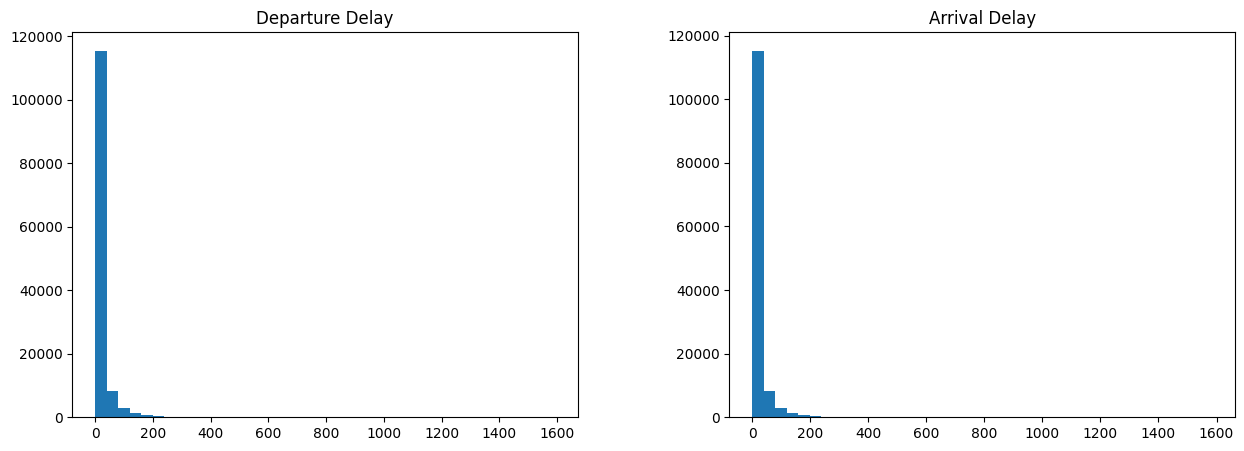
\includegraphics[width=0.9\linewidth]{project_files/project_14_1.png}
\caption{Distribution of Departure and Arrival Delays}
\end{figure}

From the above tables we can observe the following statistical characteristics of the arrival and departure delays:

\begin{itemize}
    \item {Arrival Delays:}
    \begin{itemize}
        \item {The mean arrival delay is 15.09 minutes, with a median of 0 minutes, indicating that half of the passengers arrive on time. }
        \item {75\% of the passengers arrive within 13 minutes of their scheduled arrival time, and 90\% within 44 minutes.}
        \item {The arrival delay distribution is highly skewed to the right (skewness = 6.68), indicating that only a few flights experience significant delays.}
    \end{itemize}
    \item {Departure Delays: }
    \begin{itemize}
        \item {The mean departure delay is 14.71 minutes, with a median of 0 minutes, implying that half of the passengers depart on schedule.}
        \item {75\% of the passengers depart within 12 minutes of their scheduled departure time, and 90\% within 44 minutes.}
        \item {Similar to arrival delays, the departure delay distribution is highly skewed to the right (skewness = 6.82), indicating a limited number of flights experiencing substantial delays.}
    \end{itemize}
\end{itemize}


These findings suggest that the majority of passengers experience minimal delays, with only a few flights encountering significant delays. The highly skewed distribution indicates an asymmetric pattern in the data, aligning with our observations from the provided distribution plots. These insights provide a valuable understanding of our flight punctuality and can aid in identifying areas for improvement to enhance passenger satisfaction and operational efficiency.


\begin{table}[!h]
    \centering
    \begin{tabular}{|c|c|c|}
        \hline
        &  Departure Delay & Arrival Delay \\
        \hline
        Departure Delay   &   1449.41  &  1404.21 \\
        \hline
        Arrival Delay     &   1404.21  &  1475.13 \\
        \hline
    \end{tabular}
    \caption{Covariance between Departure and Arrival Delays}
    \label{tab:cov}
\end{table}

The arrival and departure delays exhibit a strong linear relationship, as evidenced by their pairwise covariance of 1404.20 and a high Pearson correlation coefficient of 0.96. This robust correlation indicates that changes in one variable are highly predictive of corresponding changes in the other. As expected, the arrival delay, representing the variance between the actual and scheduled arrival time, closely corresponds to the departure delay, which captures the variance between the actual and scheduled departure time. This interdependence between the two delay metrics underscores their potential utility in predicting each other's outcomes, enabling us to gain valuable insights for optimizing flight scheduling and operational efficiency.

\begin{table}[!h]
    \centering
    \begin{tabular}{|c|c|c|}
        \hline 
        &  Departure Delay & Arrival Delay \\
        \hline
        Departure Delay   &   1.00  &  0.96 \\
        \hline
        Arrival Delay     &   0.96  &  1.00 \\
        \hline
    \end{tabular}
    \caption{Pearson correlation between Departure and Arrival Delays}
    \label{tab:corr}
\end{table}
    
The real meaning of these two numbers is that the pilots are not able to make up the delays during the flight, and that the delays are caused by the ground operations.


    
\hypertarget{discretization-of-nominal-features}{%
\section{Discretization of nominal
features}\label{discretization-of-nominal-features}}


The histograms of the age, flight distance, departure delay, and arrival delay attributes reveal some interesting characteristics about the airline's customer base and operations. The majority of passengers are between the ages of 16 and 55, around 45,000 youth and 60,000 middle aged passengers. This suggests that the airline's target market is mostly adults, corporate working age travelers. 

The flight distance distribution is normal, which suggests that the airline operates a large number of medium-haul flights, but also almost the same amounts of long and short-haul flights. This is partially true, since there is approximately 4 times as many short flights as long, and 8 times as many medium distance flights.

The departure delay distribution is geometric, with it's peak at the "Short" delays. The arrival delay distribution is almost a carbon copy of the departure distribution, with it's peak at the "Short" as well. This suggests that the airline is overwhelmingly good at arriving and departing on time.

Overall, the histograms suggest that the airline is doing a good job of covering it's customer base, and both arriving and departing on time for a large majority of times. However, there is still room for improvement in terms of departure and arrival delays. The age distribution could be used to segment the customer base and target marketing campaigns accordingly. The satisfaction distribution could be used to identify areas where the airline could improve its customer service. The flight distance distribution could be used to optimize the airline's route network and fleet composition. The departure delay distribution could be used to identify which flights are most likely to be delayed and take steps to mitigate those delays. The arrival delay distribution could be used to identify which airports are most likely to experience delays and take steps to improve those airports' operations.


    \begin{figure}[h]
\centering
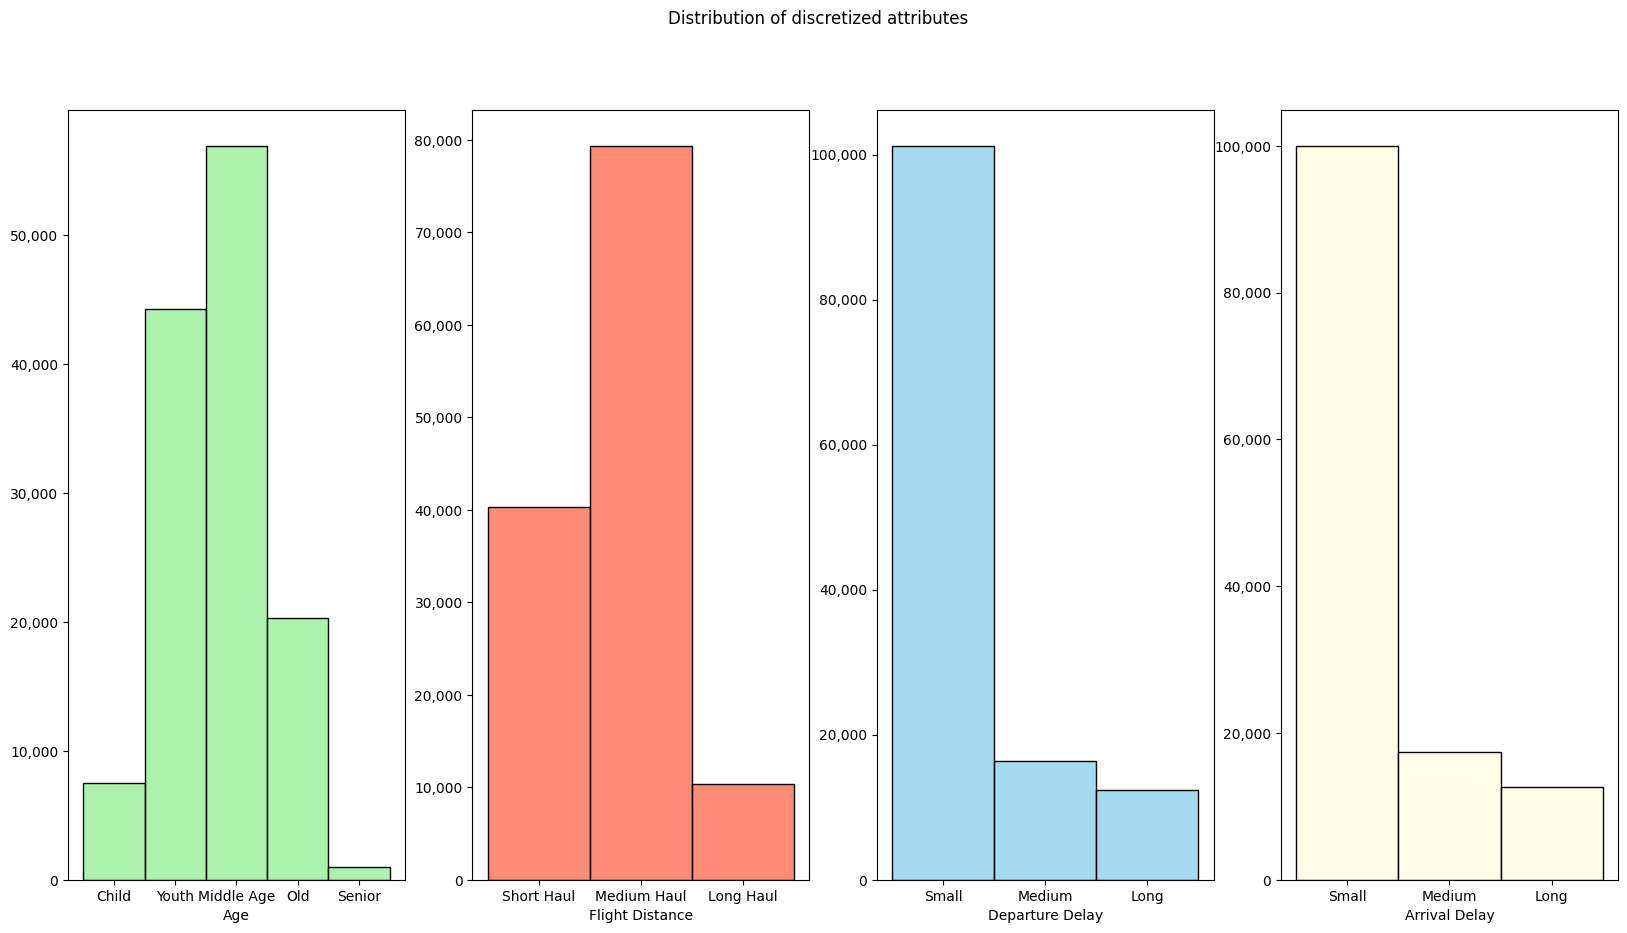
\includegraphics[width=0.7\linewidth]{project_files/project_20_1.png}
\caption{Distribution of discretized features}
\end{figure}

        
    \hypertarget{question-3}{%
\section{Hypothesis Testing}\label{question-3}}

\subsection{Long haul passengers’ overall satisfaction is influenced more by the in-flight service quality than by the departure delays.}

To test the given hypothesis, we first had to calculate the Pearson correlation coefficient between in-flight services and satisfaction as well as departure delays and satisfaction. Depending on the results, if the coefficient is closer to 1 the more linear the relationship between them is, and the close the number is to 0 the more negligible the relationship between the two variables is. 

\begin{table}[!h]
    \centering
    \begin{tabular}{|c|c|c|}
        \hline
        &  In-flight Service & Satisfaction (0-1) \\
        \hline
        In-flight Service   &   1.00  &  0.52 \\
        \hline
        Satisfaction (0-1)     &   0.52  &  1.00 \\
        \hline
    \end{tabular}
    \caption{Correlation between in-flight service and satisfaction}
    \label{tab:corr-ifs-s}
\end{table}

As observed from the table above, the correlation coefficient between the in-flight service and overall satisfaction is \num{0.52}, showing a moderate linear relationship between the two attributes. To investigate this further, the two attributes were processed through a linear regression model, which outputted the plot shown below.

\begin{figure}[h]
\centering
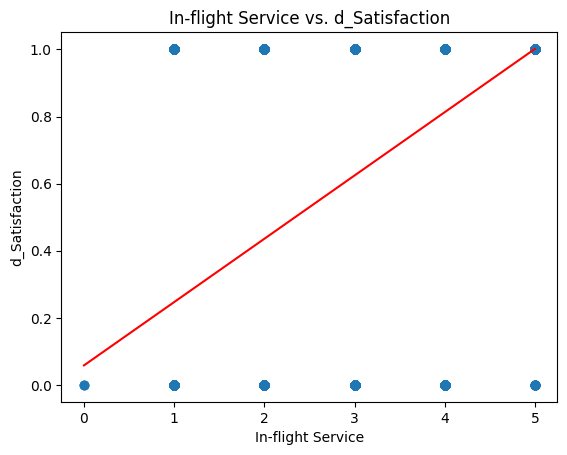
\includegraphics[width=0.5\linewidth]{project_files/project_21_1.png}
\caption{Linear relationship between in-flight service and satisfaction}
\end{figure}

In comparison, when calculating the correlation coefficient between departure delay and overall satisfaction, we were able to observe the values presented in the table below. The coefficient being \num{-0.08}, means there is almost no relationship between the two variables and even the slight correlation is negative. This however makes perfect sense since the longer the departure delay is the lower the passenger is likely to rate overall satisfaction with the airline.

\begin{table}[!h]
    \centering
    \begin{tabular}{|c|c|c|}
        \hline
        &  Departure Delay & Satisfaction (0-1) \\
        \hline
        Departure Delay   &   1.00  &  -0.08 \\
        \hline
        Satisfaction (0-1)     &   -0.08  &  1.00 \\
        \hline
    \end{tabular}
    \caption{Correlation between departure delay and satisfaction}
    \label{tab:corr-depd-s}
\end{table}

To make it easier to visualize the relationship between the variables, the below plot was created. The circle marks on the y axis represent the overall satisfaction with the airline services and the x axis represents the departure delay experienced by the passenger. As we can clearly see, the satisfaction regression line (in red) has a negative slope \num{-0.0009}, meaning that for each minute added in departure the likeliness of getting a satisfied score decreases by the slope number.

\begin{figure}[h]
\centering
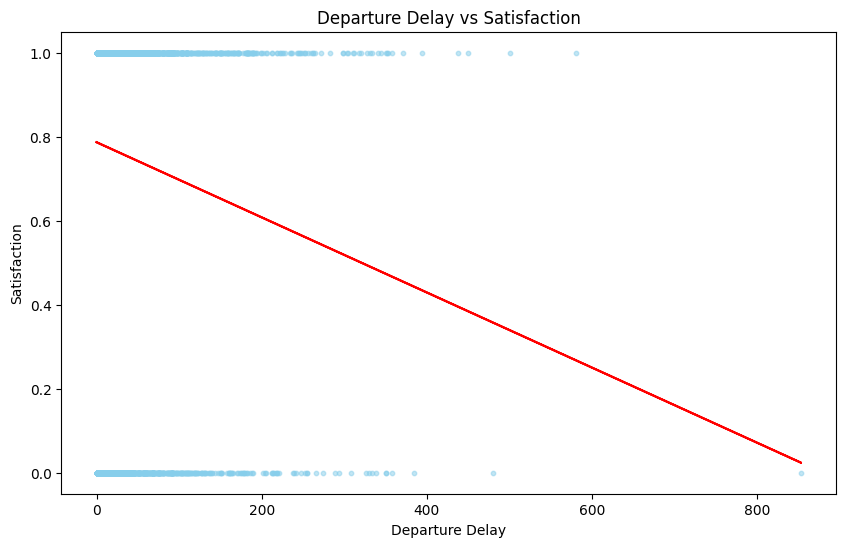
\includegraphics[width=0.5\linewidth]{project_files/project_21_2.png}
\caption{Linear relationship between departure delay and satisfaction}
\end{figure}
    
Overall, we can confidently say that in-flight services influence the passenger's satisfaction rating a lot more than experiencing departure delays. This has been proven through comparing the correlation coefficients as well as comparing the linear regression slopes. 

\subsection{Medium haul passengers’ overall satisfaction is influenced more by the arrival delays than by the in-flight entertainment.}

In order to evaluate the given hypothesis, it was imperative to initially compute the Pearson correlation coefficient between the in-flight entertainment and satisfaction, as well as arrival delays and satisfaction. Based on the outcome, if the coefficient tends towards 1, it indicates a stronger linear association between the variables, whereas a coefficient closer to 0 signifies a weaker or negligible relationship between the two variables.
        
\begin{table}[!h]
    \centering
    \begin{tabular}{|c|c|c|}
        \hline
        &  In-flight Entertainment & Satisfaction (0-1) \\
        \hline
        In-flight Entertainment     &   1.00  &  0.40 \\
        \hline
        Satisfaction (0-1)     &   0.40 & 1.00 \\
        \hline
    \end{tabular}
    \caption{Correlation between in-flight entertainment delay and satisfaction}
    \label{tab:corr-ife-s}
\end{table}

From the above table we were able to observe that the correlation between in-flight entertainment and passenger satisfaction is \num{0.40} making the two attributes moderately correlated in a linear fashion. This is further proven by the regression plot that is shown below.

    \begin{figure}[h]
\centering
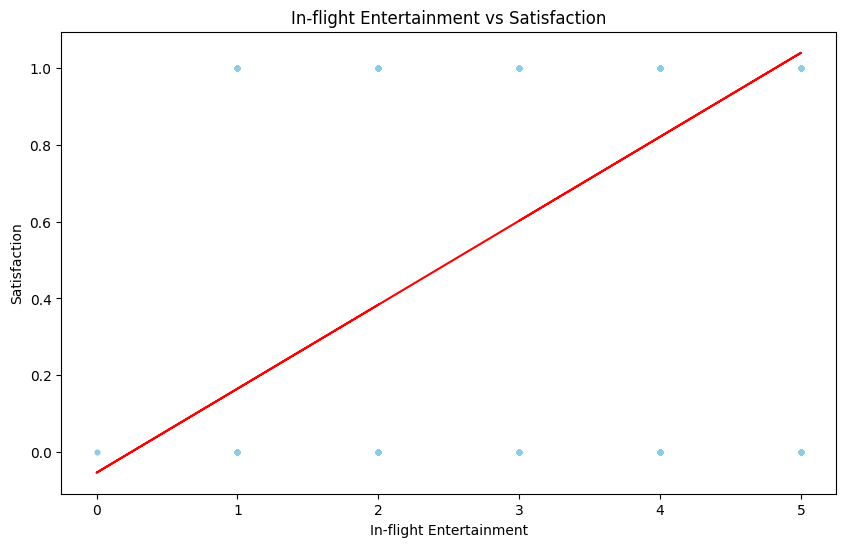
\includegraphics[width=0.5\linewidth]{project_files/project_22_1.png}
\caption{Linear relationship between in-flight entertainment and satisfaction}
\end{figure}

Plotting the regression line gave us the slope and intercept values of the line \num{0.22} and \num{-0.05} respectively. 

\begin{table}[!h]
    \centering
    \begin{tabular}{|c|c|c|}
        \hline
        &  Arrival Delay & Satisfaction (0-1) \\
        \hline
        Arrival Delay     &   1.00  &  -0.05 \\
        \hline
        Satisfaction (0-1)     &   -0.05 & 1.00 \\
        \hline
    \end{tabular}
    \caption{Correlation between arrival delay and satisfaction}
    \label{tab:corr-arrd-s}
\end{table}

To complete the comparison, we calculated the correlation coefficient between arrival delay and overall satisfaction rating. This calculation resulted in a value of \num{-0.05} which shows a negligible relationship between the two attributes. The negative part of the number is a natural pattern since the longer the arrival delay is the lower the satisfaction rating is predicted to be. 

\begin{figure}[h]
\centering
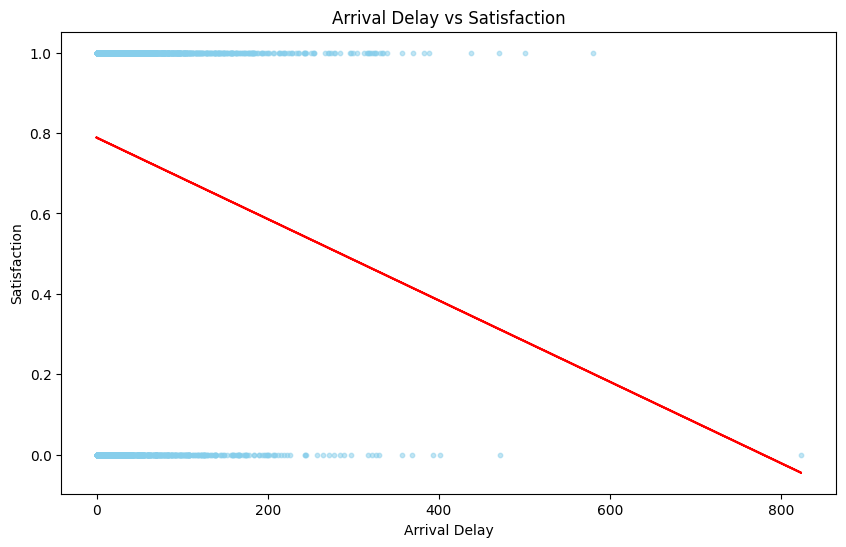
\includegraphics[width=0.5\linewidth]{project_files/project_22_2.png}
\caption{Linear relationship between arrival delay and satisfaction}
\end{figure}

The above stated natural pattern can be observed through the negative regression line that is plotted in red on the scatter plot below. In this visualization the marks represent the individual arrival delays, while the regression line is the predicted line along which the passenger scores their overall satisfaction. In conclusion, in-flight entertainment services offered by the airline influence the overall satisfaction rating much more than arrival delays do, which was proven through the comparison of correlation coefficients and comparing regression slopes.
        
\subsection{Medium and short-haul passengers' overall satisfaction is influenced more by Online boarding than by either in-flight wifi service or the in-flight entertainment}

In order to test the hypothesis, we first had to merge the passengers who are both medium and short-haul flights, and reduce the scope of the other attributes to In-flight wifi, in-flight entertainment, online boarding and overall satisfaction. The purpose of this hypothesis is to prove that both in-flight services are more important to passengers than the online boarding process offered, when measured in attribute correlation. 

\begin{table}[!h]
    \centering
    \begin{tabular}{|c|c|c|c|c|}
        \hline
        &  In-Flight WiFi &  In-Flight Entertainment & Online Boarding & Satisfaction \\
        \hline
        In-flight WiFi     &   1.00  &  0.21 & 0.49 & 0.30 \\
        \hline
In-flight Entertainment     &   0.21 & 1.00 & 0.27 &  0.38 \\
        \hline
        Online Boarding     &   0.49 & 0.27 & 1.00 & 0.49 \\
        \hline
        Satisfaction     &   0.30 & 0.38 & 0.49 & 1.00 \\
        \hline
    \end{tabular}
    \caption{Correlation between in-flight wifi, entertainment, online boarding and satisfaction}
    \label{tab:corr-ifw-ife-ob-s}
\end{table}

From the above table we can observe that the attributes most to least correlated to overall satisfaction rating are online boarding, in-flight entertainment, and in-flight wifi respectively. It is extremely surprising to see that online boarding is value higher than either services when considering overall satisfaction rating. 

To further compare the attributes we conducted a comparison between the regression slopes and found that the highest slope was between in-flight entertainment and satisfaction (\num{0.22}) and the second highest between online boarding and satisfaction (\num{0.18}). This means that both of these two attributes have a higher linear relationship than in-flight wifi and satisfaction, which has a slope of (\num{0.04}). 

In conclusion, through complex data analysis we were able to prove that medium and short-haul passengers don't value either wifi or entertainment services as highly as online boarding, and are much more likely to be satisfied with their flight when either wifi or entertainment services meet their expectations.
    
    \hypertarget{question-4}{%
\section{Association rules between attributes}\label{question-4}}

In this comprehensive analysis, we meticulously examined several crucial attributes that play a pivotal role in shaping the aviation industry's dynamics. The attributes considered for investigation encompassed Gender, Age, Type of travel, Flight distance, Class, Arrival delays, and Overall satisfaction. Applying sophisticated association rule mining techniques to a vast dataset, we successfully unearthed ten highly significant associations characterized by a minimum support threshold of 100 and a minimum confidence level of 60\%. These association rules epitomize the intricate relationships between different variables, revealing invaluable patterns and tendencies within the aviation domain.

Of particular significance, the associations predominantly centered around the attributes of age, gender, and type of travel, shedding light on the potential interdependencies and preferences of diverse passenger segments. By delving into the interplay between these vital demographic factors and other variables like class, flight distance, and arrival delays, we can glean remarkable insights into passenger behaviors, expectations, and satisfaction levels.

The depth and breadth of our association rule analysis offer decision-makers and industry stakeholders a solid foundation for strategic planning, marketing initiatives, and service enhancement efforts. Armed with this knowledge, airlines, travel agencies, and industry professionals can devise tailored strategies to cater to the unique needs and preferences of various passenger groups, ensuring heightened customer satisfaction and bolstered business performance.

Furthermore, our findings transcend the realm of mere statistical analysis, transforming into actionable intelligence that holds the potential to revolutionize the way aviation entities engage with their clientele. Whether optimizing flight offerings, personalizing passenger experiences, or crafting targeted marketing campaigns, the application of these association rules will undoubtedly pave the way for enhanced operational efficiency and a competitive edge in an ever-evolving industry landscape.


\begin{table}[!h]
    \centering
    \begin{tabular}{|c|c|c|c|c|}
        \hline
        If &  Then &  Support & Confidence & Zhang's Metric \\
        \hline
        Age = Child     &   Type of Travel = Personal  &  0.043 & 0.76 & 0.63 \\
        \hline
        Age = Child     &   Class = Economy & 0.042 & 0.74 &  0.41 \\
        \hline
        Age = Child     &   Flight Distance = Medium Haul & 0.038 & 0.66 & 0.08 \\
        \hline
        Gender = Female     &   Type of Travel = Business & 0.352 & 0.69 & 0.01 \\
        \hline
        Gender = Male     &   Arrival Delay = Small  &  0.390 & 0.77 & 0.0004 \\
        \hline
        Gender = Female     &   Arrival Delay = Small  &  0.378 & 0.77 & -0.0004 \\
        \hline
    \end{tabular}
    \caption{\centering Association rules between Gender, Age, Type of travel, Flight distance, Class, Arrival delays, and Overall satisfaction.}
    \label{tab:ar}
\end{table}

The analysis of association rules presented in the above table brings forth a notable observation wherein the child age group emerges as a significant driver in the majority of rule formations. A deeper examination of the rules reveals a coherent and natural pattern, suggesting that children are predominantly inclined to travel for personal reasons, opting for economy class and medium flight distances. Remarkably, this singular pattern encompasses a substantial portion of our dataset, aligning well with the high confidence scores and Zhang's metric score.

An illustrative example from the table emphasizes this point. Considering the rule \emph{"Age = Child"} implying \emph{"Type of Travel = Personal"}, it surfaces in 4\% of the dataset. However, what sets this rule apart is the impressive 76\% confidence level, indicating that the consequent (then-part) of the rule frequently occurs within all the groups that share the antecedent (if-part).

Such compelling insights derived from the association rules analysis hold the potential to shape strategic decisions within the aviation domain significantly. By recognizing the distinctive travel preferences of children, airlines and travel service providers can tailor their offerings to enhance overall customer satisfaction and retention. Additionally, this knowledge equips industry stakeholders with a powerful data-driven approach to optimize marketing endeavors, personalize customer experiences, and efficiently allocate resources based on passenger demographics and preferences.

        
    \hypertarget{question-5}{%
\section{Feature Scaling}\label{question-5}}

In this data analysis and data mining project for our airline company, we utilized Principal Component Analysis (PCA) to combine features A10-A23 into a single feature named PCAS. By computing the average (AVES), minimum (MINS), and maximum (MAXS) values for each passenger record in A10-A23, we gained insights into the overall trends and variations in these attributes.

To better understand passenger satisfaction, we converted the "overall satisfaction" feature, A24, into a numeric value (DA24) by representing neutral or unsatisfied responses as 1.0 and satisfied responses as 4.0.

\begin{table}[!h]
    \centering
    \begin{tabular}{|c|c|c|c|c|}
        \hline
        PCAS &  AVES &  MINS & MAXS & DA24 \\
        \hline
        -2.793 & 3.413 & -2.793  & 5.0  &   0 \\
        \hline
        -2.618 & 3.358 & -2.618  & 5.0  &   4 \\
        \hline
        -2.684 & 3.487 & -2.684  & 5.0  &   4 \\
        \hline
        -2.623 & 3.358 & -2.623  & 5.0  &   4 \\
        \hline
        -1.319 & 3.178 & -1.319  & 5.0  &   4 \\
        \hline
    \end{tabular}
    \caption{Principal Component Analysis (n = 1) with instance based mean, min, and max values.}
    \label{tab:pca}
\end{table}

Our findings indicate that the instance-based average values ranged from 1.535 to 4.258, while the minimum values ranged from -6.128 to 2.000, and the maximum values ranged from 3.000 to 8.116. The PCA magnitude, obtained with one component count, was also within this range of -6.128 to 8.116.

\begin{figure}[h]
\centering
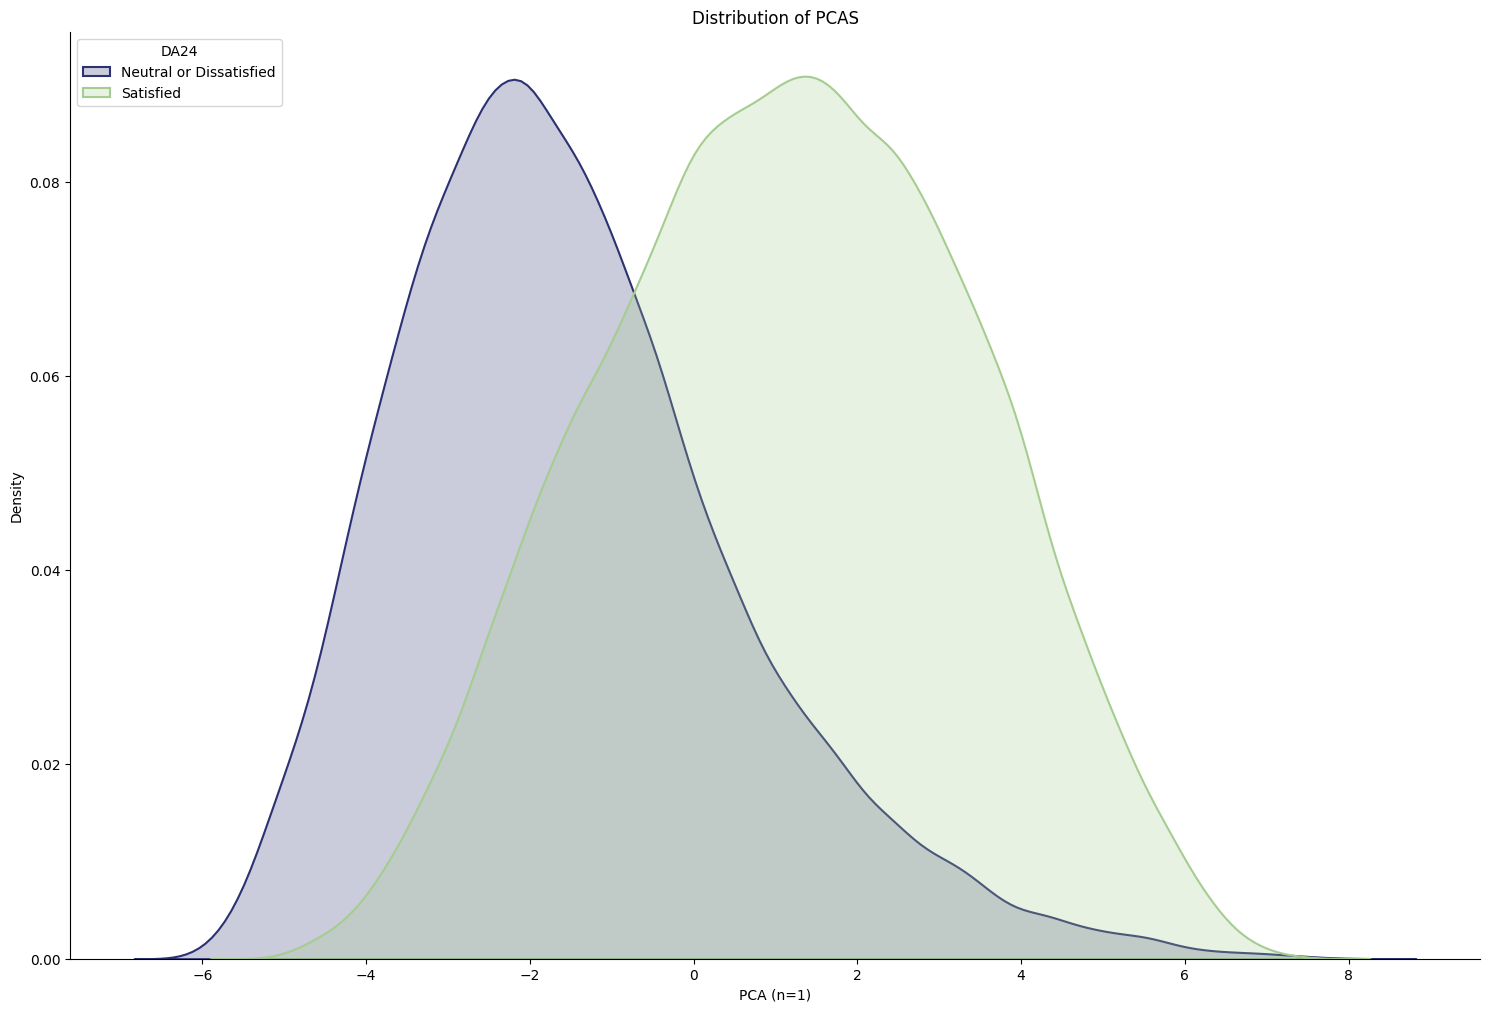
\includegraphics[width=0.7\linewidth]{project_files/project_37_0.png}
\caption{\centering Kernel Density Estimation of PCA \emph{(n=1)} component highlighted based on passenger satisfaction}
\end{figure}

When exploring the relationship between PCA values and passenger satisfaction (DA24), we observed a consistent pattern: the class value (DA24) displayed a uniform change along the negative slope of the PCA values. Moreover, the Kernel Density Estimation (KDE) plot revealed a distinct distribution of neutral or dissatisfied customers (purple bell curve) to the left side of the x-axis (negative PCA values), while satisfied customers (green bell curve) were more densely positioned along the positive x-axis values.

The Pearson correlation coefficient analysis unveiled valuable insights into the associations between various attributes and passenger satisfaction. Specifically, we found a moderate negative correlation (-0.519840) between PCAS and passenger satisfaction (DA24). Additionally, the correlation values between mean values (AVES), minimums (MINS), and maximums (MAXS) with passenger satisfaction were 0.478688, -0.543850, and 0.252245, respectively.

Understanding these relationships empowers our airline company to make data-driven decisions that enhance customer experiences, ultimately leading to increased overall customer satisfaction and loyalty. The PCA-derived PCAS and instance-based calculations (AVES, MINS, and MAXS) play pivotal roles in evaluating and improving passenger satisfaction, allowing us to maintain a competitive edge in the market and foster enduring customer relationships.

\subsection{Principal Component Analysis using 3 components}

In our analysis using Principal Component Analysis (PCA), we transformed features A10-A23 into three new features named PCAS, PCAS1, and PCAS2. These components allowed us to capture essential patterns in the data efficiently. After conducting the analysis, we computed the average, minimum, and maximum values for A10-A23 for each passenger instance, which we refer to as AVES, MINS, and MAXS, respectively. The instance-based average values ranged between 1.495 and 3.592, while the minimum values ranged from -6.128 to 1.639, and the maximum values ranged from 3.000 to 8.116.

\begin{table}[!h]
    \centering
    \begin{tabular}{|c|c|c|c|c|c|c|}
        \hline
        PCAS & PCAS2 & PCAS3 &  AVES &  MINS & MAXS & DA24 \\
        \hline
        -2.793 &  1.328 &  0.845 & 3.139 & -2.793  & 5.0  &   0 \\
        \hline
        -2.618 &  2.452 & -1.761 & 3.004 & -2.618  & 5.0  &   4 \\
        \hline
        -2.684 & -1.248 &  2.658 & 3.160 & -2.684  & 5.0  &   4 \\
        \hline
        -2.623 &  2.733 & -1.589 & 3.030 & -2.623  & 5.0  &   4 \\
        \hline
        -1.319 &  0.101 &  1.684 & 2.909 & -1.319  & 5.0  &   4 \\
        \hline
    \end{tabular}
    \caption{Principal Component Analysis (n = 3) with instance based mean, min, and max values.}
    \label{tab:pca2}
\end{table}

Our PCA results revealed that the magnitude of the first component fell within the range of -6.128 to 8.116, the second component ranged from -5.958 to 6.702, and the third component ranged from -5.564 to 6.151. By plotting these results, we observed a denser concentration of values between -4 and 4 for each component. This is clearly shown in the kernel density estimation (KDE) plot, where the purple bell curve represents Neutral or Dissatisfied customers, and the green bell curve represents Satisfied customers.

The first component exhibited a normal distribution for both satisfied and dissatisfied customers, with dissatisfied customers tending to have negative values and satisfied customers tending to have positive values. The second component's density distribution showed that neutral and dissatisfied customers had a lower density but a wider bell curve with multiple peaks, while satisfied customers were densely concentrated along the 0 and -2 x-axis range. As for the final component's density distribution, both Neutral or Dissatisfied and Satisfied customers were equally densely populated between the -2 and 2 x-axis values, with both bell curves having almost equally tall and wide peaks. Only a small fraction of the neutral or dissatisfied population was dense outside of these values.

\begin{figure}[h]
\centering
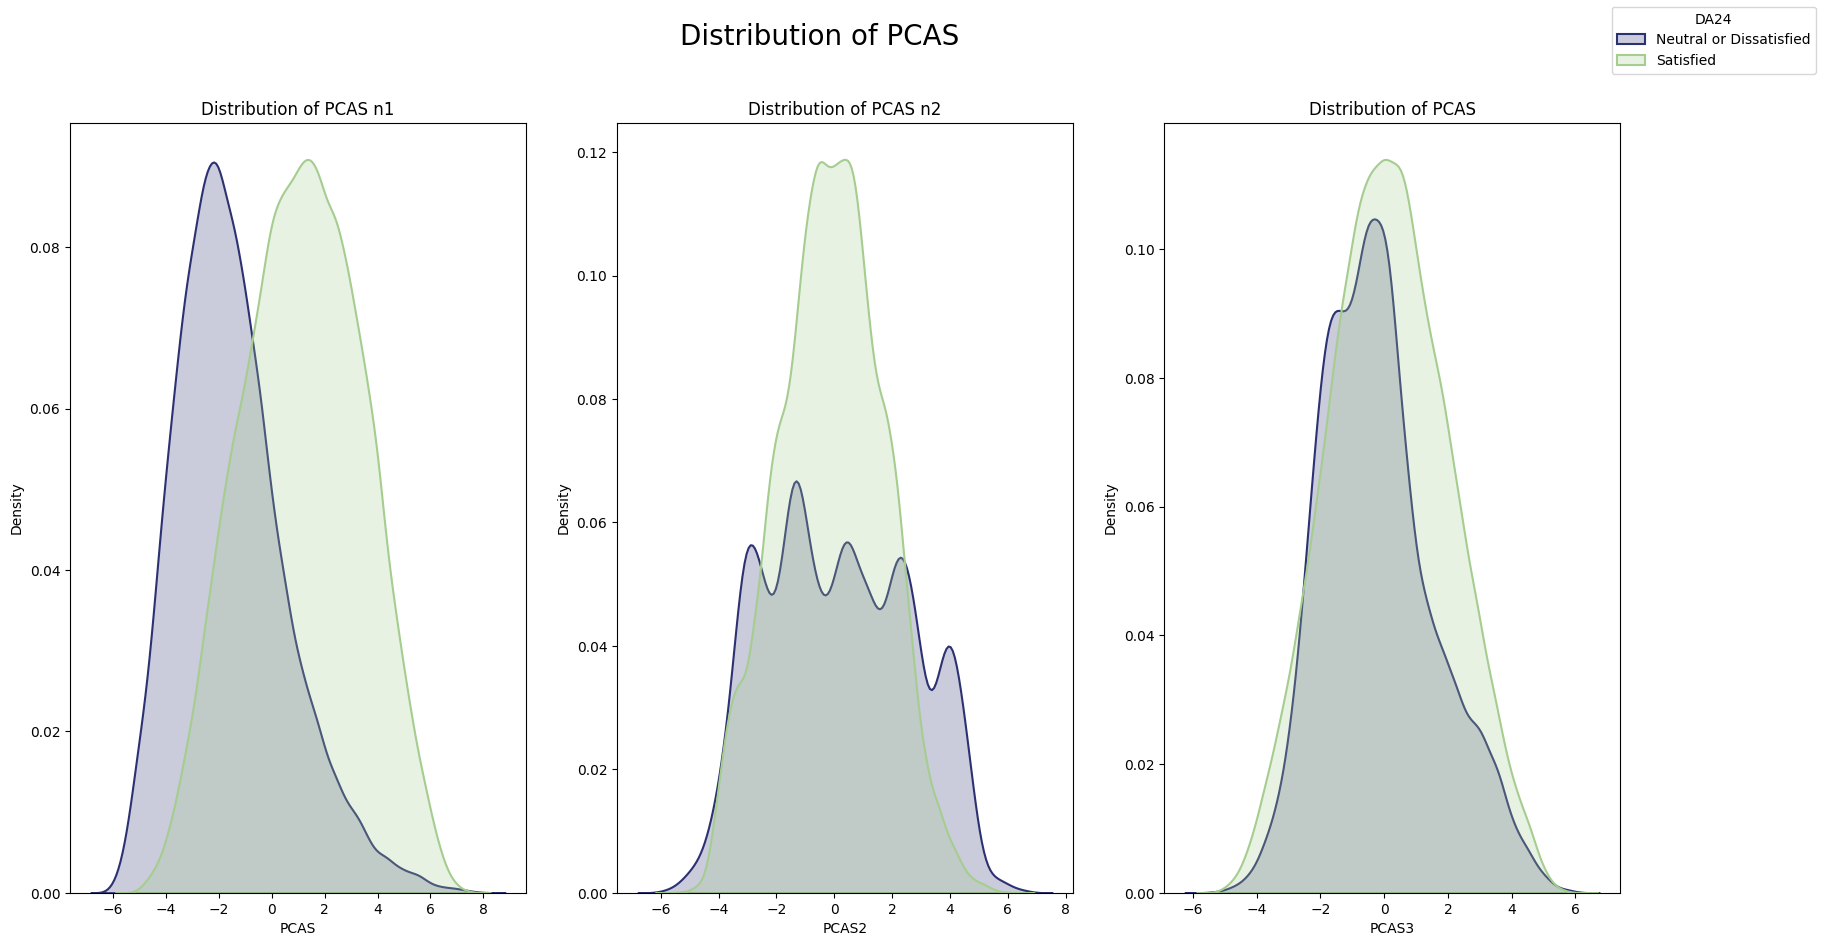
\includegraphics[width=0.9\linewidth]{project_files/project_37_1.png}
\caption{
\centering
Kernel Density Estimation of each PCA \emph{(n=3)} component highlighted based on passenger satisfaction}
\end{figure}

Furthermore, our three-dimensional plot confirmed the same pattern, with the majority of the population falling within the -2 and 2 values on all axes. Moving on to the correlation analysis, we calculated the Pearson correlation coefficient between the class labels (DA24) and the magnitude values of the PCA components, as well as the instance-based calculations (AVES, MINS, MAXS). The correlations between PCA component 1 and the class label, PCA component 2 and the class label, and the last PCA component and the class label were -0.519840, 0.064479, and -0.090071, respectively.

\begin{figure}[h]
\centering
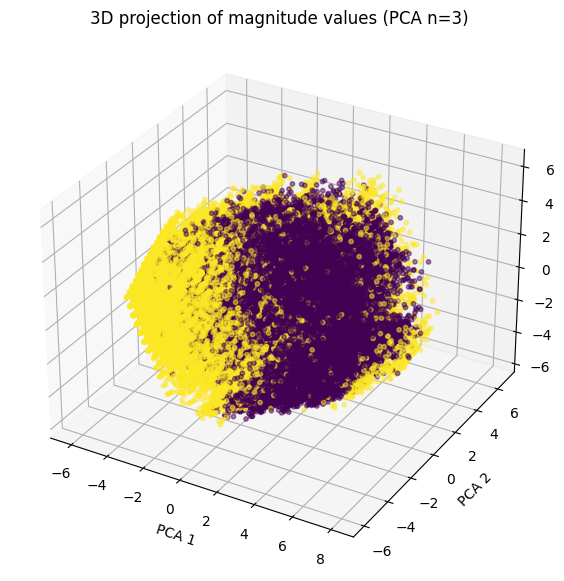
\includegraphics[width=0.5\linewidth]{project_files/project_38_0.png}
\caption{3D projection of each PCA component's magnitude}
\end{figure}

Additionally, we found correlations of 0.493949 between the mean values and the class label, -0.337138 between the minimum values and the class label, and 0.255260 between the maximum values and the class label. These correlations provide insights into how the PCA components and instance-based calculations relate to customer satisfaction levels, thereby aiding in understanding key factors influencing overall satisfaction.


    
    \hypertarget{question-6}{%
\section{Regression Modeling}\label{question-6}}
\subsection{Arrival Delay and Flight Distance}

In our analysis of the relationship between flight distance and arrival delay, we found that the majority of delays fall within the range of 0 to 20 minutes, with 75\% of passengers experiencing a delay of only 13 minutes. However, when conducting linear regression modeling, we observed no significant relationship between arrival delays and flight distances. The derived model yielded an R-squared score of 0.00000373, indicating an extremely weak correlation. Additionally, the mean squared error was found to be 1475.11, with a mean absolute error of 20.38.

\begin{table}[!h]
    \centering
    \begin{tabular}{|c|c|}
            \hline
            Evaluation &  Score \\
            \hline
            $R^2$   &    \num{3.73e-06} \\
            \hline
            MSE     &   1475.11  \\
            \hline
            MAE     &   20.38  \\
            \hline
            MAPE     &    \num{3.80e+16}  \\
            \hline
    \end{tabular}
    \caption{\centering Evaluation results of the Linear Regression model}
    \label{tab:lr-1-eval}
\end{table}

Despite the lack of a strong relationship, we were able to calculate the coefficients and intercept values for the linear model, which were found to be -0.0000744 and 15.18, respectively. Plotting the regression line revealed a nearly horizontal orientation. Moreover, our predictive analysis showed that for a flight distance of 500 miles, the approximate arrival delay would be 15.14 minutes, while flights of 1000 and 2000 miles would result in delays of around 15.10 and 15.03 minutes, respectively.

\begin{center}
    $f_{(\text{arrival delay})} = \num{-7.44e-05} * distance + 15.18$
\end{center}

Based on these results, it is evident that flight distance has a negligible and negative impact on arrival delays. As flight distance increases, the arrival delay decreases only marginally, suggesting that other factors might be more influential in determining delays. It is essential for our airline company to consider these findings when planning and managing flight schedules. While optimizing routes and minimizing flight distances can potentially lead to slightly shorter delays, our focus should also be on identifying and addressing other contributing factors to enhance overall punctuality and passenger satisfaction.

\begin{table}[!h]
    \centering
    \begin{tabular}{|c|c|}
            \hline
            Flight Distance (miles) &  Predicted Arrival Delay (minutes) \\
            \hline
            500   &   15.14 \\
            \hline
            1000     &   15.10  \\
            \hline
            2000     &   15.03  \\
            \hline
            3000     &   14.95  \\
            \hline
    \end{tabular}
    \caption{\centering Predicted arrival delays based on flight distance in miles}
    \label{tab:lr-1-eval}
\end{table}

In conclusion, the linear regression modeling indicates a limited relationship between flight distance and arrival delay. Our analysis suggests that the majority of delays are attributed to factors beyond flight distance. As a result, our company should explore comprehensive strategies to improve on-time performance and customer experience, including advanced operational planning, efficient ground services, and effective communication with air traffic control and other stakeholders. By taking a holistic approach, we can better position our airline to deliver exceptional service and maintain a competitive edge in the industry.

\begin{figure}[h]
\centering
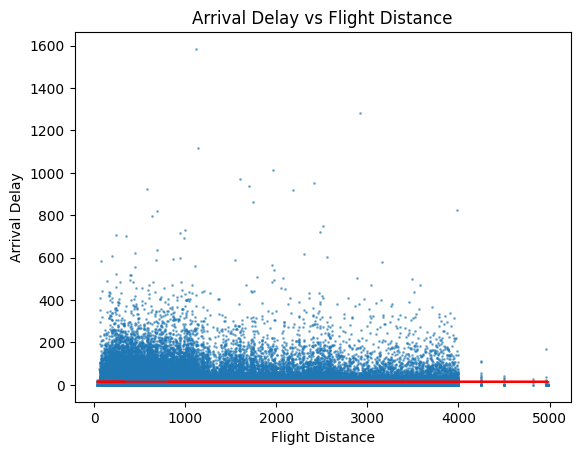
\includegraphics[width=0.5\linewidth]{project_files/project_40_1.png}
\caption{Regression Line showing negligible relationship between arrival delays and flight distance}
\end{figure}
    
    \subsection{Departure Delay and Flight Distance}

Our analysis of the relationship between flight distance and departure delay revealed that the distribution of departure delays is skewed towards smaller delays, with the majority falling within the 0 to 20-minute range. This observation is consistent with various points highlighted throughout this document, including the mean distribution of departure delays and the quartile separation, where we found that 75\% of passengers experience a departure delay of only 12 minutes. These findings suggest that most flights exhibit minimal departure delays, creating a favorable scenario for our airline's punctuality and passenger satisfaction.

\begin{center}
    $f_{(\text{departure delay})} = \num{9.16e-05} * distance + 14.60$
\end{center}

However, upon conducting linear regression modeling to explore the relationship between departure delays and flight distances, we discovered no significant correlation between the two attributes. The derived model yielded a positive R-squared score of 0.00000576, indicating an extremely weak relationship. Additionally, the mean squared error of 1449.29 and the mean absolute error of 20.15 further supported the absence of a substantial association between departure delays and flight distances. Despite this outcome, we were able to determine the coefficient and intercept values of the linear model, which were found to be 0.0000916 and 14.60, respectively.

\begin{table}[!h]
    \centering
    \begin{tabular}{|c|c|}
            \hline
            Evaluation &  Score \\
            \hline
            $R^2$   &    \num{5.77e-06} \\
            \hline
            MSE     &   1449.39  \\
            \hline
            MAE     &   20.15  \\
            \hline
            MAPE     &    \num{3.74e+16}  \\
            \hline
    \end{tabular}
    \caption{\centering Evaluation results of the Linear Regression model}
    \label{tab:lr-2-eval}
\end{table}

Plotting the regression line reaffirmed the lack of a clear relationship, with the line appearing almost horizontal. The predicted departure delays for different flight distances further demonstrated this negligible correlation. For instance, a flight distance of 500 miles resulted in an approximate departure delay of 14.65 minutes, while flights of 1000 and 2000 miles exhibited delays of 14.69 and 14.78 minutes, respectively. These slight variations in predicted departure delays suggest that flight distance has minimal impact on departure delays, and other factors are likely more influential in determining the departure schedule.


\begin{figure}[h]
\centering
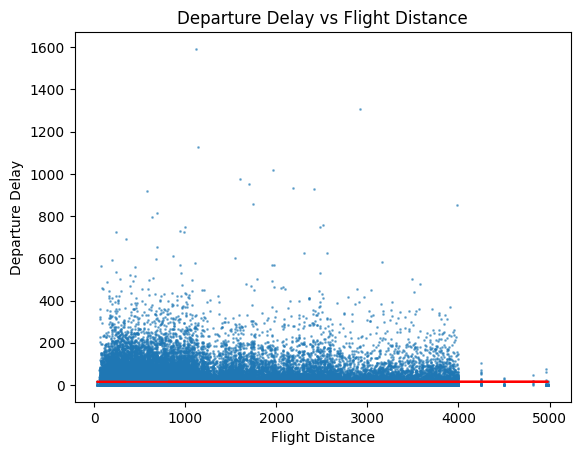
\includegraphics[width=0.5\linewidth]{project_files/project_41_1.png}
\caption{\centering Regression Line showing negligible relationship between departure delays and flight distance}
\end{figure}

While the absence of a significant relationship between flight distance and departure delays might appear unexpected, it also presents an opportunity for our airline. By focusing on other factors affecting departure delays, such as ground operations, boarding processes, and air traffic control coordination, we can strategically optimize our operations to enhance departure punctuality. Furthermore, the negligible relationship discovered in the regression analysis allows us to concentrate on refining other aspects of the flying experience, such as in-flight services and customer engagement, to create a positive and memorable journey for our passengers. By leveraging these insights and diversifying our approach to address various delay factors, we can position our airline as a leader in the industry and ensure an exceptional travel experience for our valued customers.

\begin{table}[!h]
    \centering
    \begin{tabular}{|c|c|}
            \hline
            Flight Distance (miles) &  Predicted Departure Delay (minutes) \\
            \hline
            500   &   14.65 \\
            \hline
            1000     &   14.69  \\
            \hline
            2000     &   14.78  \\
            \hline
            3000     &   14.87  \\
            \hline
    \end{tabular}
    \caption{\centering Predicted departure delays based on flight distance in miles}
    \label{tab:lr-2-eval}
\end{table}

Given that neither of the regression models revealed a distinct relationship between the delays and flight distances, I took the initiative to explore an alternative analysis. In the upcoming section, I independently modeled the relationship between arrival delays and departure delays. This investigation aims to shed light on whether a connection exists between the time an aircraft departs and the time it arrives at its destination. Understanding such relationships could offer valuable insights into our operational efficiency and identify areas where improvements can be made to minimize overall travel time for passengers.


\subsection{Departure Delay and Arrival Delay}
Our analysis of the relationship between departure delays and arrival delays using linear regression revealed a highly significant linear correlation between the two attributes. The model exhibited an impressive R-squared score of 0.922, indicating a close-to-perfect correlation between departure and arrival delays. Moreover, the mean squared error of 112.71 and mean absolute error of 5.26 further validated the accuracy and precision of the derived model. These results suggest that our regression model effectively captures the relationship between departure and arrival delays, providing valuable insights into their interdependency.

\begin{center}
        $f_{(\text{departure delay})} = 0.95 * \text{arrival delay} + 0.34$
\end{center}

The coefficients and intercept values calculated for the linear model were found to be 0.951 and 0.348, respectively. These coefficients indicate that for each minute of delay in departure, there is a corresponding increase of approximately 0.951 minutes in arrival delay. The positive intercept value of 0.348 represents the delay that occurs when the departure delay is zero. This implies that even if a flight departs on time, a small delay may still occur upon arrival. The positive nature of both the coefficients and intercept aligns with our intuitive understanding that longer departure delays will lead to longer arrival delays, assuming no adjustments can be made in flight.

\begin{table}[!h]
    \centering
    \begin{tabular}{|c|c|}
        \hline
        Evaluation &  Score \\
        \hline
        $R^2$   &    0.92 \\
        \hline
        MSE     &   112.71  \\
        \hline
        MAE     &   5.26  \\
        \hline
        MAPE     &    \num{5.43e15}  \\
        \hline
    \end{tabular}
    \caption{\centering Evaluation results of the Linear Regression model}
    \label{tab:lr-3-eval}
\end{table}

Plotting the regression line reaffirmed the positive linear relationship between departure delays and arrival delays. As the departure delay increases, the regression line shows a corresponding increase in the predicted arrival delay, creating a clear and consistent trend. For instance, the model predicted that a flight with an estimated arrival delay of 10 minutes would have an approximate departure delay of 9.867 minutes, while a flight with an estimated arrival delay of 60 minutes would have a predicted departure delay of 57.463 minutes. These predictions align with our understanding that delays in departure are likely to impact the overall arrival schedule, especially for longer delays.

\begin{table}[!h]
    \centering
    \begin{tabular}{|c|c|}
            \hline
            Arrival Delay (minutes) &  Predicted Departure Delay (minutes) \\
            \hline
            10   &   9.86 \\
            \hline
            60     &   57.46  \\
            \hline
    \end{tabular}
    \caption{\centering Predicted departure delays based on the arrival delay}
    \label{tab:lr-3-eval}
\end{table}

The strong positive relationship between departure and arrival delays in our analysis aligns with common operational challenges faced in the airline industry. Delays in departure often have a cascading effect on the entire travel schedule, as subsequent flights may experience congestion and scheduling adjustments to accommodate late arrivals. Understanding this relationship is crucial for effective flight planning and resource allocation. By identifying the interdependency between departure and arrival delays, our airline can develop proactive strategies to minimize overall delays, enhance operational efficiency, and ultimately improve customer satisfaction.

\begin{figure}[h]
\centering
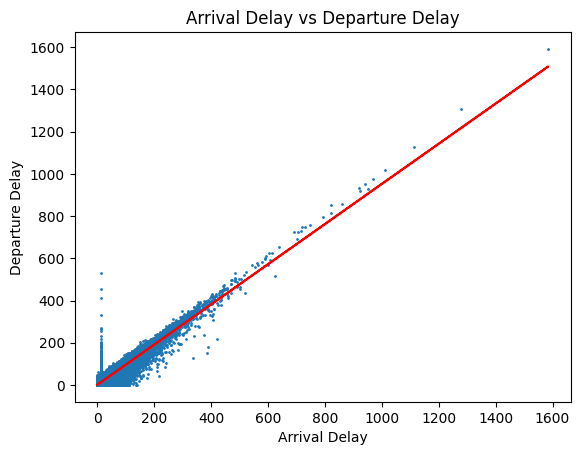
\includegraphics[width=0.5\linewidth]{project_files/project_42_1.png}
\caption{\centering Regression Line showing strong linear relationship between departure delays and arrival delays}
\end{figure}

The insights derived from the regression model can be leveraged to optimize our airline's performance and minimize the impact of delays on the passenger experience. Implementing real-time monitoring and adaptive scheduling can help us respond quickly to departure delays, minimizing their effects on subsequent flights and mitigating the ripple effect. Moreover, we can explore opportunities to streamline ground operations and improve turnaround times to reduce departure delays and enhance punctuality. By proactively managing both departure and arrival delays, we can enhance our reputation for reliability and provide our passengers with a seamless and enjoyable travel experience.

    
    \hypertarget{question-7}{%
\section{Satisfaction Correlations}\label{question-7}}

    \hypertarget{question-7.1}{%
\subsection{Is satisfaction with seat comfort related (or depends on) to passenger Gender?}\label{question-7.1}}

In analyzing the data, we focused on exploring potential relationships between different attributes. Specifically, we examined the connection between passenger gender and seat comfort ratings. The results indicate that both females and males rated seat comfort similarly, with average ratings of 3.48 and 3.40, respectively.

\begin{table}[!h]
    \centering
    \begin{tabular}{|c|c|c|}
        \hline
        Gender & Seat Comfort & Satisfaction \\
        \hline
        Female  &    3.481   &     0.428 \\
        \hline
        Male  &    3.400   &     0.440 \\
        \hline
    \end{tabular}
    \caption{\centering Mean rating of seat comfort and overall satisfaction for each gender}
    \label{tab:7-1}
\end{table}

Moreover, it is worth noting that the gender of the passenger did not seem to influence the overall satisfaction rating given by the passengers. Approximately 42\% of female passengers and 44\% of male passengers reported being satisfied, suggesting that satisfaction levels are comparable between both sexes.

\begin{figure}[h]
\centering
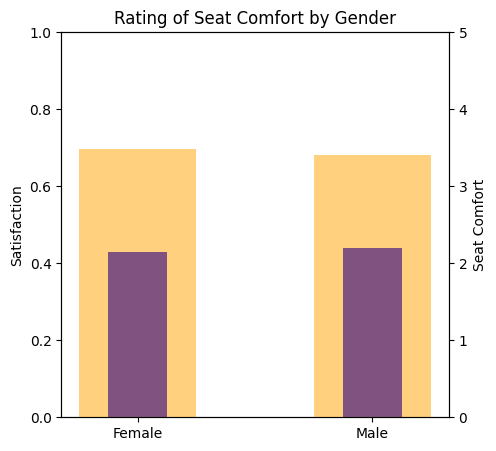
\includegraphics[width=0.3\linewidth]{project_files/project_50_0.png}
\caption{\centering Rating of seat comfort by both genders along with overall satisfaction probability}
\end{figure}

Furthermore, a correlation analysis between passenger gender and average seat comfort rating was conducted. The coefficient value derived from this analysis was \num{0.03}, which is considered negligible. This suggests that there is no significant correlation between the two variables – gender and seat comfort rating.

\begin{table}[!h]
    \centering
    \begin{tabular}{|c|c|c|}
        \hline
        &  Gender  & Seat Comfort \\
        \hline
        Gender    &  1.000    &  0.031 \\
        \hline
        Seat Comfort & 0.031    &  1.000 \\
        \hline
    \end{tabular}
    \caption{\centering Pearson correlation coefficient}
    \label{tab:7-1-2}
\end{table}

Finally, we performed a Linear Regression analysis on the two target variables, namely, discretized gender and seat comfort. The results of this analysis showed a p-value of \num{1.455e-28}, an $R^2$ value of \num{0.0009}, and a slope of \num{0.081}. These values indicate that there is no significant dependency or correlation between gender and seat comfort.

\begin{table}[!h]
    \centering
    \begin{tabular}{|c|c|}
        \hline
        R\^{}2:    & 0.0009 \\
        \hline
        P-value:   & \num{1.455e-28} \\
        \hline
        std. error:& 0.0073 \\
        \hline
        intercept: & 3.4002 \\
        \hline
        slope:     & 0.0812 \\
        \hline
    \end{tabular}
    \caption{\centering Regression modeled on Seat Comfort and passenger Gender}
    \label{tab:7-1-3}
\end{table}

In conclusion, the data suggests that seat comfort ratings are not influenced by passenger gender and that the online booking experience has a more notable impact on seat comfort levels. This information can help us understand passenger preferences and potentially inform strategies to enhance overall customer satisfaction and comfort during flights.

        
%     From the above table we can see that both females, and males rate seat
% comfort similarly, 3.48 and 3.40 average rating respectively.
% Furthermore, the gender of the passenger does not impact the overall
% satisfaction rating given by the passenger as both sexes were satisfied
% approximately 42\% for females and 44\% for males of the time.

        
%     When directly analyzing the correlation between passenger gender and
% average seat comfort rating, we are able to see that they have a
% coefficient value of 0.03 which is considered negligible. This means
% that there is no correlation between the two variables. If we reference
% the above heatmap, we can see that Seat Comfort is most closely
% correlated with the Online Booking experience with a coefficient value
% of 0.42 which is considered to be a significant correlation.

%     After running Linear Regression analysis on the two target variables
% (discretized gender, and seat comfort), we found a p-value of
% \emph{1.4551e-28}, an r-square value of \emph{0.0009} and a slope of
% \emph{0.081}. All of which indicates to no significant dependency or
% correlation between the two variables.

    \hypertarget{question-7.2}{%
\subsection{Is satisfaction with gate location related to passenger
age?}\label{question-7.2}}

Upon analyzing the data, we observed interesting trends related to the different age groups and their satisfaction ratings. The Senior age group rated Gate Location highest among all age groups, while the Child age group rated Gate Location the lowest. This discrepancy could potentially be attributed to the fact that the Child age group places more emphasis on in-flight entertainment and food options rather than the Gate Location.

\begin{table}[!h]
    \centering
    \begin{tabular}{|c|c|c|}
        \hline
        Age & Gate Location  & Satisfaction \\
        \hline
    Senior  &     3.019        & 0.296 \\
        \hline
Middle Age  &     2.987        & 0.547 \\
        \hline
     Youth  &     2.978        & 0.356 \\
        \hline
    Old  &     2.951        & 0.401 \\
        \hline
    Child  &     2.951        & 0.146 \\
        \hline
    \end{tabular}
    \caption{\centering Mean rating of Gate Location and percentage of overall Satisfaction for each age group sorted by Gate Location.}
    \label{tab:7-2-1}
\end{table}

Of particular note is the overall satisfaction of the Senior age group, which stands at around 29\%, making it the second lowest satisfaction level among all age groups. It appears that the airline might be falling short in meeting the expectations of the Senior age group in areas beyond Gate Location.

\begin{table}[!h]
    \centering
    \begin{tabular}{|c|c|c|}
        \hline
                            &   Age     &   Gate Location   \\
        \hline
            Age     &   1.0000        &     -0.0009     \\
        \hline
            Gate Location   &   -0.0009       &    1.0000   \\
        \hline
    \end{tabular}
    \caption{\centering Pearson correlation coefficient between discretized age and gate location}
    \label{tab:7-2-2}
\end{table}

In an attempt to identify any potential relationship between passenger age and the Gate Location rating received, we calculated the correlation coefficient between these two variables, resulting in a value of \num{-0.000982}. This value is exceedingly close to zero, indicating that there is no discernible relationship between age and the Gate Location rating. This finding is also supported by the linear least-squares regression line, with a nearly horizontal slope of \num{-0.0015} and a y-intercept of \num{2.9785}. These results reinforce the notion that no significant relationship exists between the passenger's age and the Gate Location rating.



To delve deeper into the differences between the satisfaction levels of the Senior and Child age groups, we analyzed the distribution of each satisfaction attribute within the Senior age group. Surprisingly, the Senior age group shows a skew towards satisfied customers (rating of 5) in all areas of satisfaction. However, upon closer examination, we noticed that the Senior age group is notably dissatisfied with the in-flight wifi service and the check-in services, as evident from their positive skewness (\num{0.03} and \num{0.05}, respectively).

\begin{figure}[h]
\centering
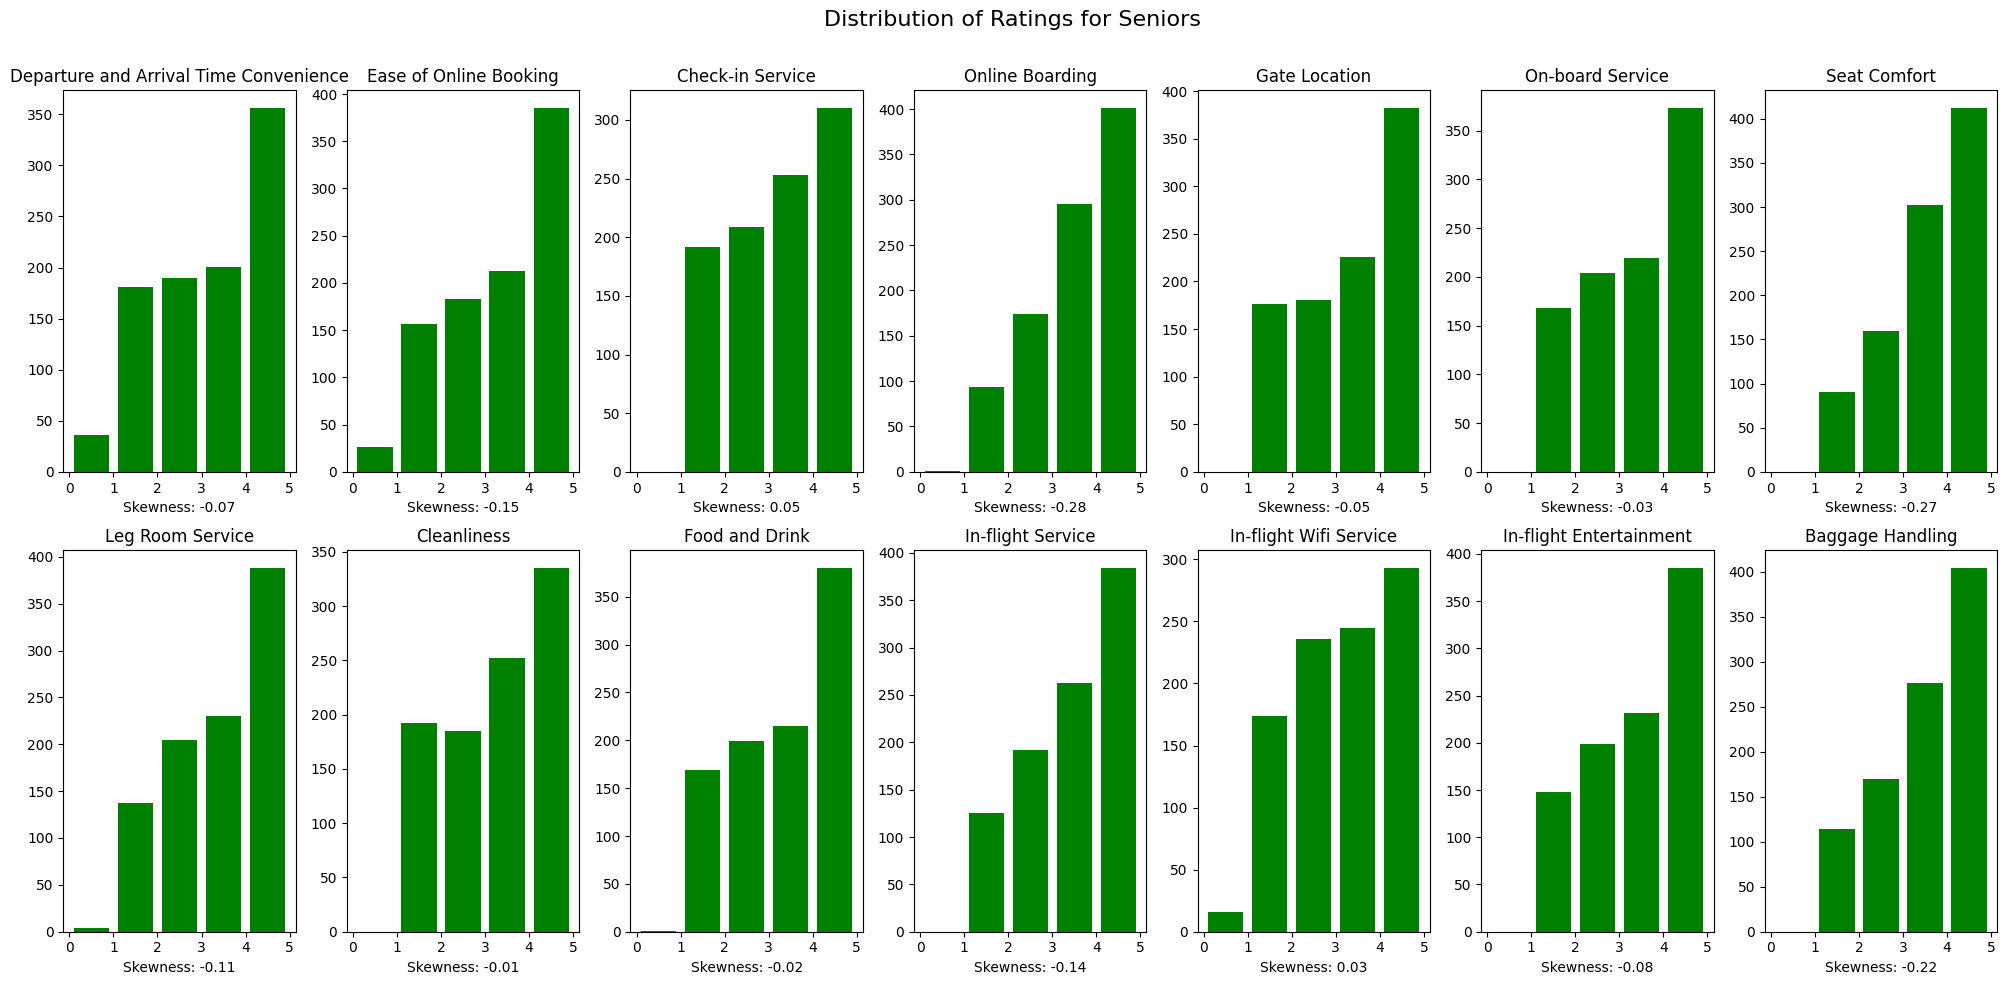
\includegraphics[width=0.9\linewidth]{project_files/project_59_0.png}
\caption{\centering Collection of histograms of each service rating of senior passengers}
\end{figure}

In conclusion, the data reveals valuable insights into the varying satisfaction levels among different age groups. The Senior age group appears to prioritize different aspects of their travel experience compared to the Child age group. Additionally, the lack of correlation between passenger age and the Gate Location rating suggests that age does not play a role in influencing this particular aspect of customer satisfaction. Understanding these trends can help the airline make informed decisions and tailor their services to meet the distinct preferences of different passenger segments, ultimately enhancing overall customer satisfaction.


        
    \hypertarget{question-7.3}{%
\subsection{Do first time passengers have more or less expectations
than returning customers measured in terms of overall
satisfaction?}\label{question-7.3}}

\begin{table}[!h]
    \centering
    \begin{tabular}{|c|c|}
        \hline
        Customer Type &     Satisfaction \\
        \hline
        Returning   &     0.478 \\
        \hline
        First-time   &     0.239 \\
        \hline
    \end{tabular}
    \caption{\centering Percentage of overall Satisfaction by Customer Type}
    \label{tab:7-3-1}
\end{table}
        
Upon analyzing the data, a noticeable disparity emerges between first time passengers and returning customers in terms of overall satisfaction. The data reveals that only 23\% of first time passengers express satisfaction with the airline's services, whereas 47\% of returning customers report being satisfied. This substantial difference in satisfaction levels can likely be attributed to returning customers being more accustomed to the services provided by the airline, leading to lower expectations compared to first time passengers.

\begin{table}[!h]
    \centering
    \begin{tabular}{|c|c|c|c|}
        \hline
        Customer Type             &                         & In-flight Wifi Service  & Satisfaction \\
        \hline
        First-time                & In-flight Wifi Service  &        1.000  &       0.434 \\
        \hline
            & Satisfaction        &                0.434    &        1.000 \\
        \hline
        \hline
        Returning                 & In-flight Wifi Service  &        1.000  &       0.260 \\
        \hline
            & Satisfaction        &                0.260    &        1.000 \\
        \hline
    \end{tabular}
    \caption{\centering Pearson correlation coefficient between in-flight wifi service and overall satisfaction across all customer types}
    \label{tab:7-3-2}
\end{table}

Interestingly, both first time passengers and returning customers demonstrate a similar pattern of dissatisfaction, with the in-flight wifi service being the primary cause, closely followed by the ease of online booking. Since these two customer groups encompass the entire passenger population, it becomes evident that improving the in-flight wifi service and enhancing the ease of online booking are crucial aspects to address in order to bolster overall customer satisfaction.

\begin{figure}[h]
\centering
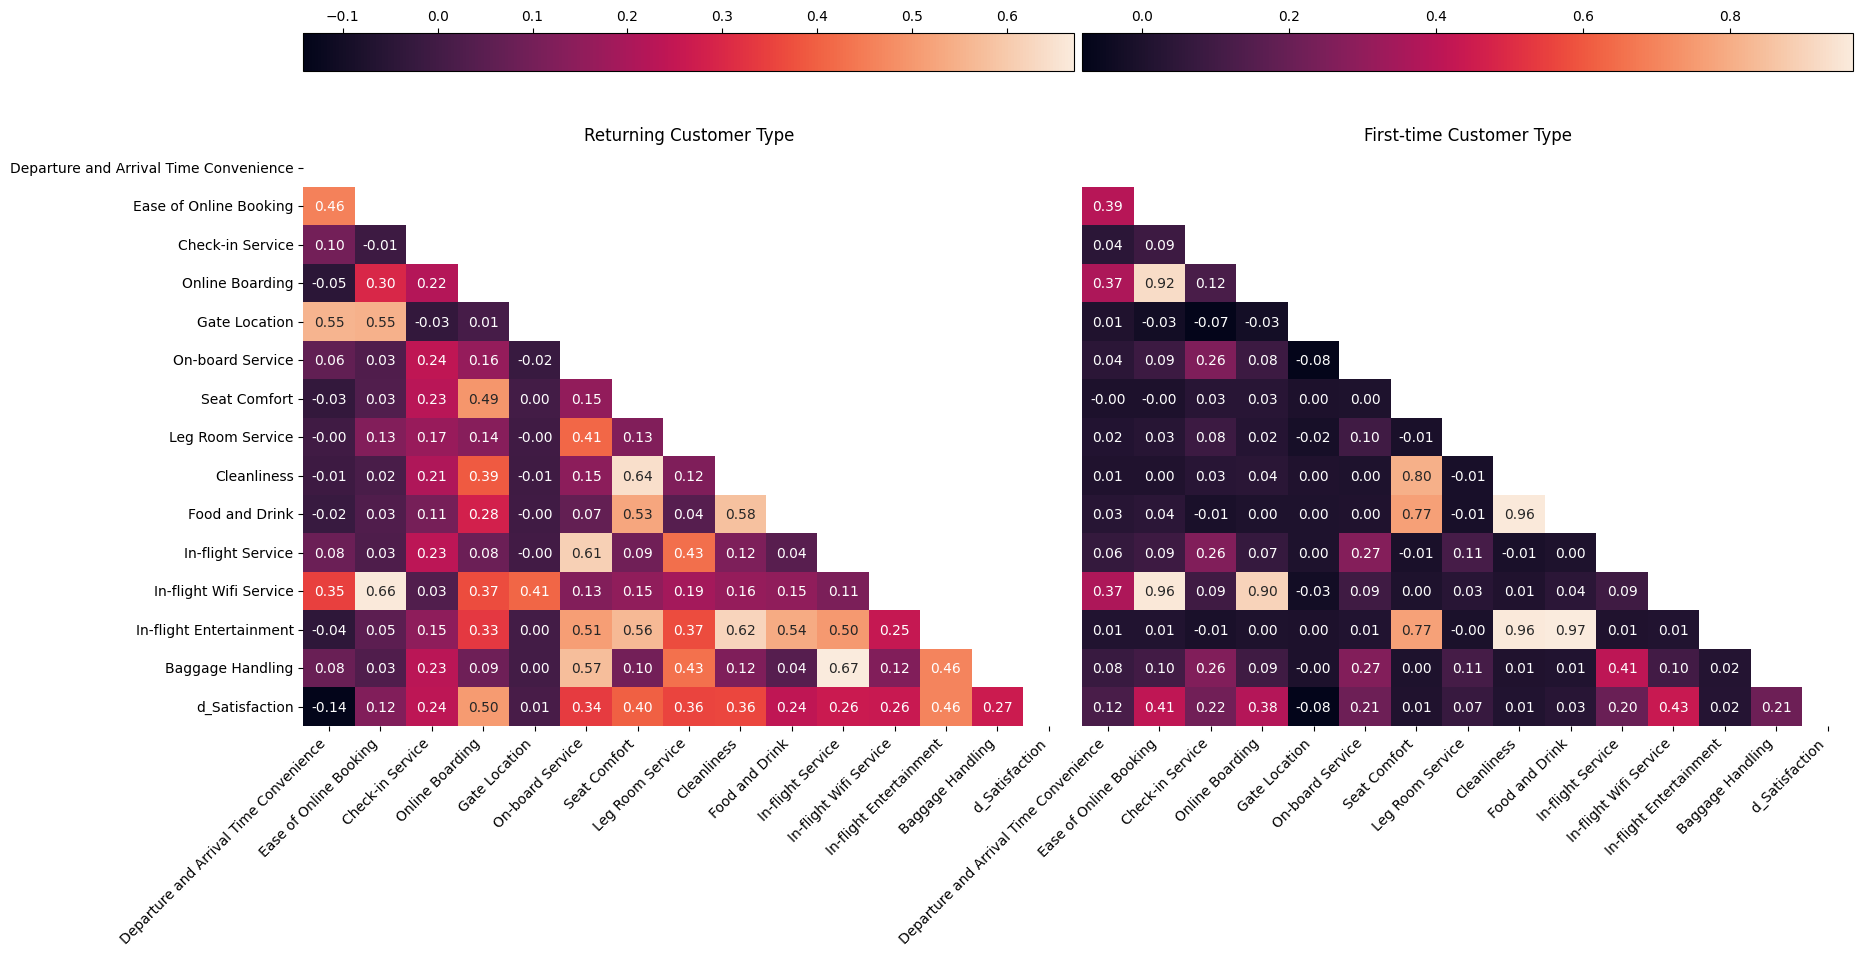
\includegraphics[width=0.9\linewidth]{project_files/project_67_1.png}
\caption{\centering Correlation matrix between services and overall satisfaction separated by customer type}
\end{figure}

In an endeavor to delve deeper into the relationship between customer types and their overall satisfaction, we conducted a thorough analysis, and the findings are presented in the three tables provided. The data highlights that first time customers' overall satisfaction exhibits a moderate correlation (correlation coefficient of \num{0.43}) with their satisfaction with the in-flight wifi service, whereas returning customers display a relatively weaker correlation (correlation coefficient of \num{0.26}). This indicates that the overall satisfaction of first time customers is significantly influenced by their level of satisfaction with the in-flight wifi service compared to returning customers.

\begin{table}[!h]
    \centering
    \begin{tabular}{|c|c|c|c|}
        \hline
        Customer Type             &                         & Ease of Online Booking & Satisfaction \\
        \hline
        First-time  &  Ease of Online Booking       &         1.000    &    0.411 \\
        \hline
              & Satisfaction               &         0.411    &    1.000 \\
        \hline
        \hline
        Returning   &  Ease of Online Booking       &         1.000    &    0.124 \\
        \hline
              & Satisfaction               &         0.124    &    1.000 \\
        \hline
    \end{tabular}
    \caption{\centering Pearson correlation coefficient between ease of online booking service rating and overall satisfaction across all customer types}
    \label{tab:7-3-2}
\end{table}

A similar trend persists when examining the Ease of Online booking service. First time customers exhibit a correlation coefficient of \num{0.41}, whereas returning customers show a correlation coefficient of \num{0.12}. These results once again underscore the fact that first time customers are more influenced by the Ease of Online booking service than returning customers when it comes to determining their overall satisfaction.

% \begin{figure}[h]
% \centering
% 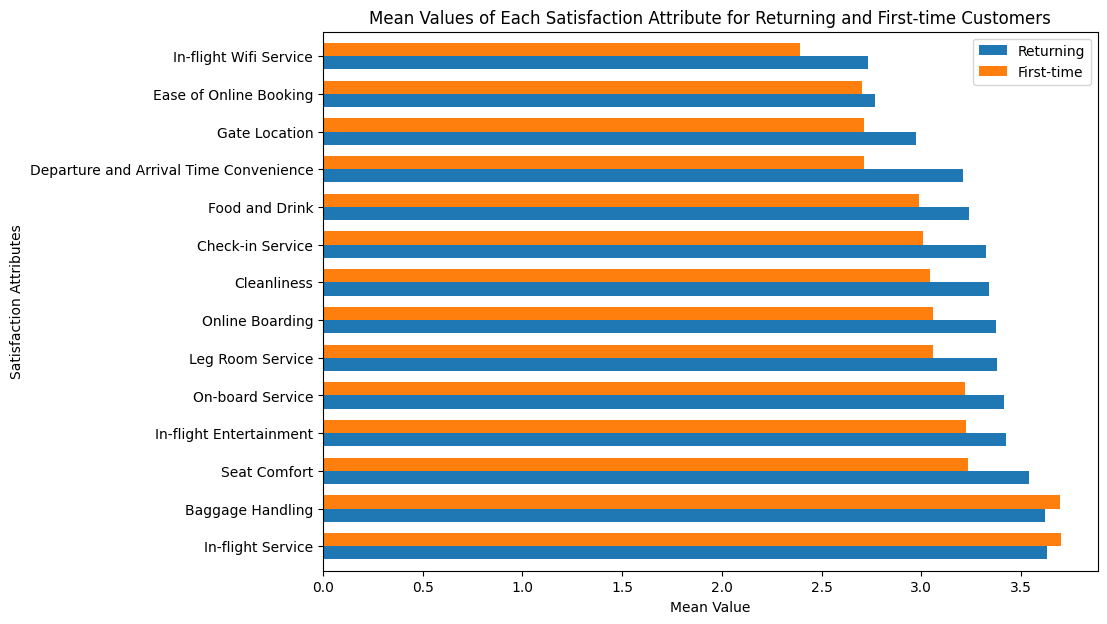
\includegraphics[width=0.9\linewidth]{project_files/project_67_0.png}
% \caption{\centering Mean values of each satisfaction attribute separated by customer type}
% \end{figure}

In conclusion, the data sheds light on the differing expectations and satisfaction levels between first time passengers and returning customers. The substantial variance in overall satisfaction suggests that the airline must pay particular attention to catering to the needs and preferences of these distinct customer groups. Focusing on enhancing the in-flight wifi service and streamlining the online booking process can prove pivotal in elevating customer satisfaction levels across the board. By understanding and addressing the specific concerns of both first time and returning customers, the airline can fortify its competitive edge and foster long-lasting customer loyalty.

    \hypertarget{question-7.4}{%
\subsection{Is there a distinct
difference between business and personal travelers in terms of their
reaction to their
flights?}\label{question-7.4}}

The satisfaction levels of Business passengers (58\%) significantly surpass those of Personal travelers (10\%). Among Business passengers, the most notable area of dissatisfaction lies in Departure and Arrival Time Convenience, where the average rating is 2.79, whereas Personal travelers provide an average rating of 3.64. This calls for further investigation by the airline to identify potential improvements that could enhance the satisfaction of Business travelers, given that they constitute twice as large a share of the passenger base.

\begin{table}[!h]
    \centering
    \begin{tabular}{|c|c|c|c|}
        \hline
                                               & Business & Personal & $\Delta$ \\
        \hline
        Departure and Arrival Time Convenience & 2.794  & 3.644 & 0.849 \\
        \hline
        Online Boarding                        & 3.455 & 2.800 & 0.654 \\
        \hline
        Ease of Online Booking                 & 2.882 & 2.476 & 0.406 \\
        \hline
        Gate Location                          & 3.002 & 2.919 & 0.082 \\
        \hline
        Check-in Service                       & 3.292 &    3.337 & 0.044 \\
        \hline
    \end{tabular}
    \caption{\centering Mean rating of 5 highest rated services by business and personal travelers.}
    \label{tab:7-4-3}
\end{table}


Upon closely examining the concatenated heatmap, we observe distinct correlation patterns between different features for each passenger travel type. Notably, Personal travelers display the highest overall correlation between any service provided by the airline and passenger satisfaction for the "In-flight wifi service," with a correlation value of 0.32. In contrast, Business travelers exhibit the highest correlation between overall satisfaction and "online boarding," with a correlation value of 0.55. Although Business travelers have larger correlations between overall satisfaction and all services, they have fewer correlations exceeding 0.7 (precisely 10 services), compared to Personal travelers who have none.


\begin{figure}[h]
\centering
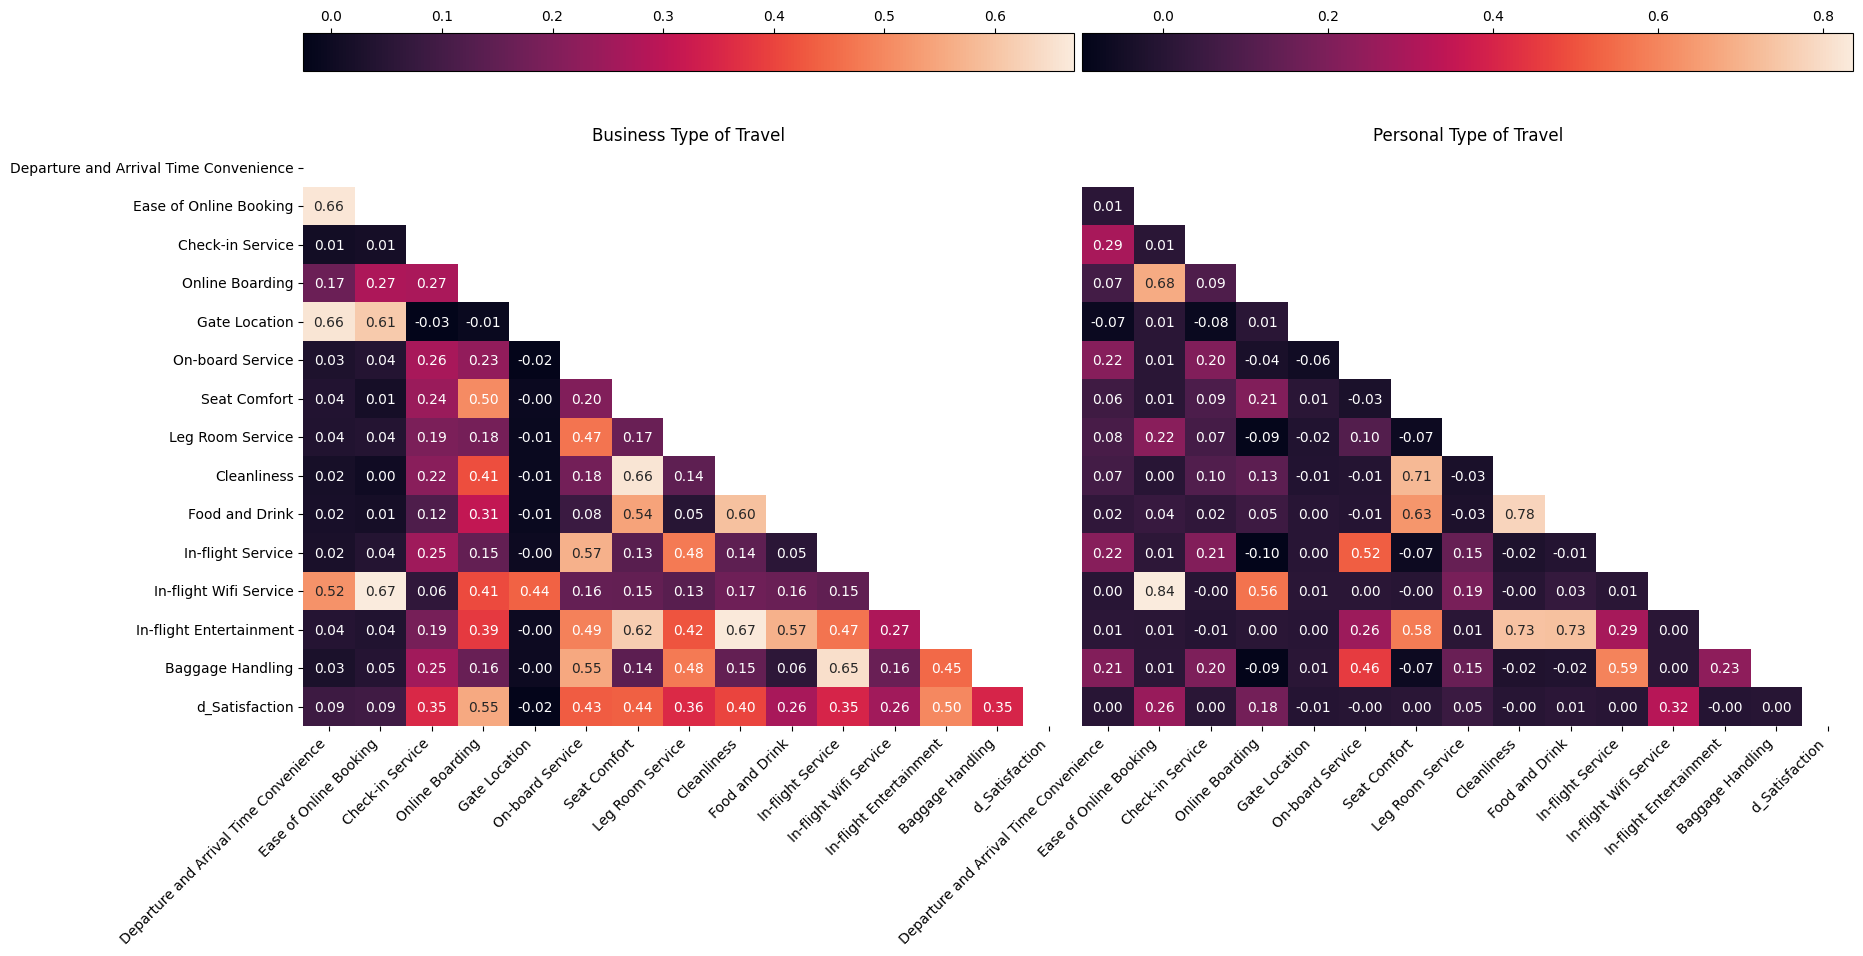
\includegraphics[width=0.9\linewidth]{project_files/project_78_0.png}
\caption{\centering Correlation matrix between services and overall satisfaction separated by traveler type}
\end{figure}


To better understand this trend, we analyzed the skewness of ratings for both passenger types. As expected, Business travelers exhibit higher skewness, indicating a greater likelihood of extreme ratings on both ends of the satisfaction scale. For example, when comparing the distribution of ratings for the in-flight entertainment service, Business travelers show a heavily skewed distribution, with over 40,000 individuals giving a rating of 5, while Personal travelers display a more uniform distribution. Specifically, the skewness for Business travelers is -0.511949, while for Personal travelers, it is -0.042002. A skewness closer to 0 suggests a more uniform distribution of ratings within the traveler group.

\begin{figure}[h]
\centering
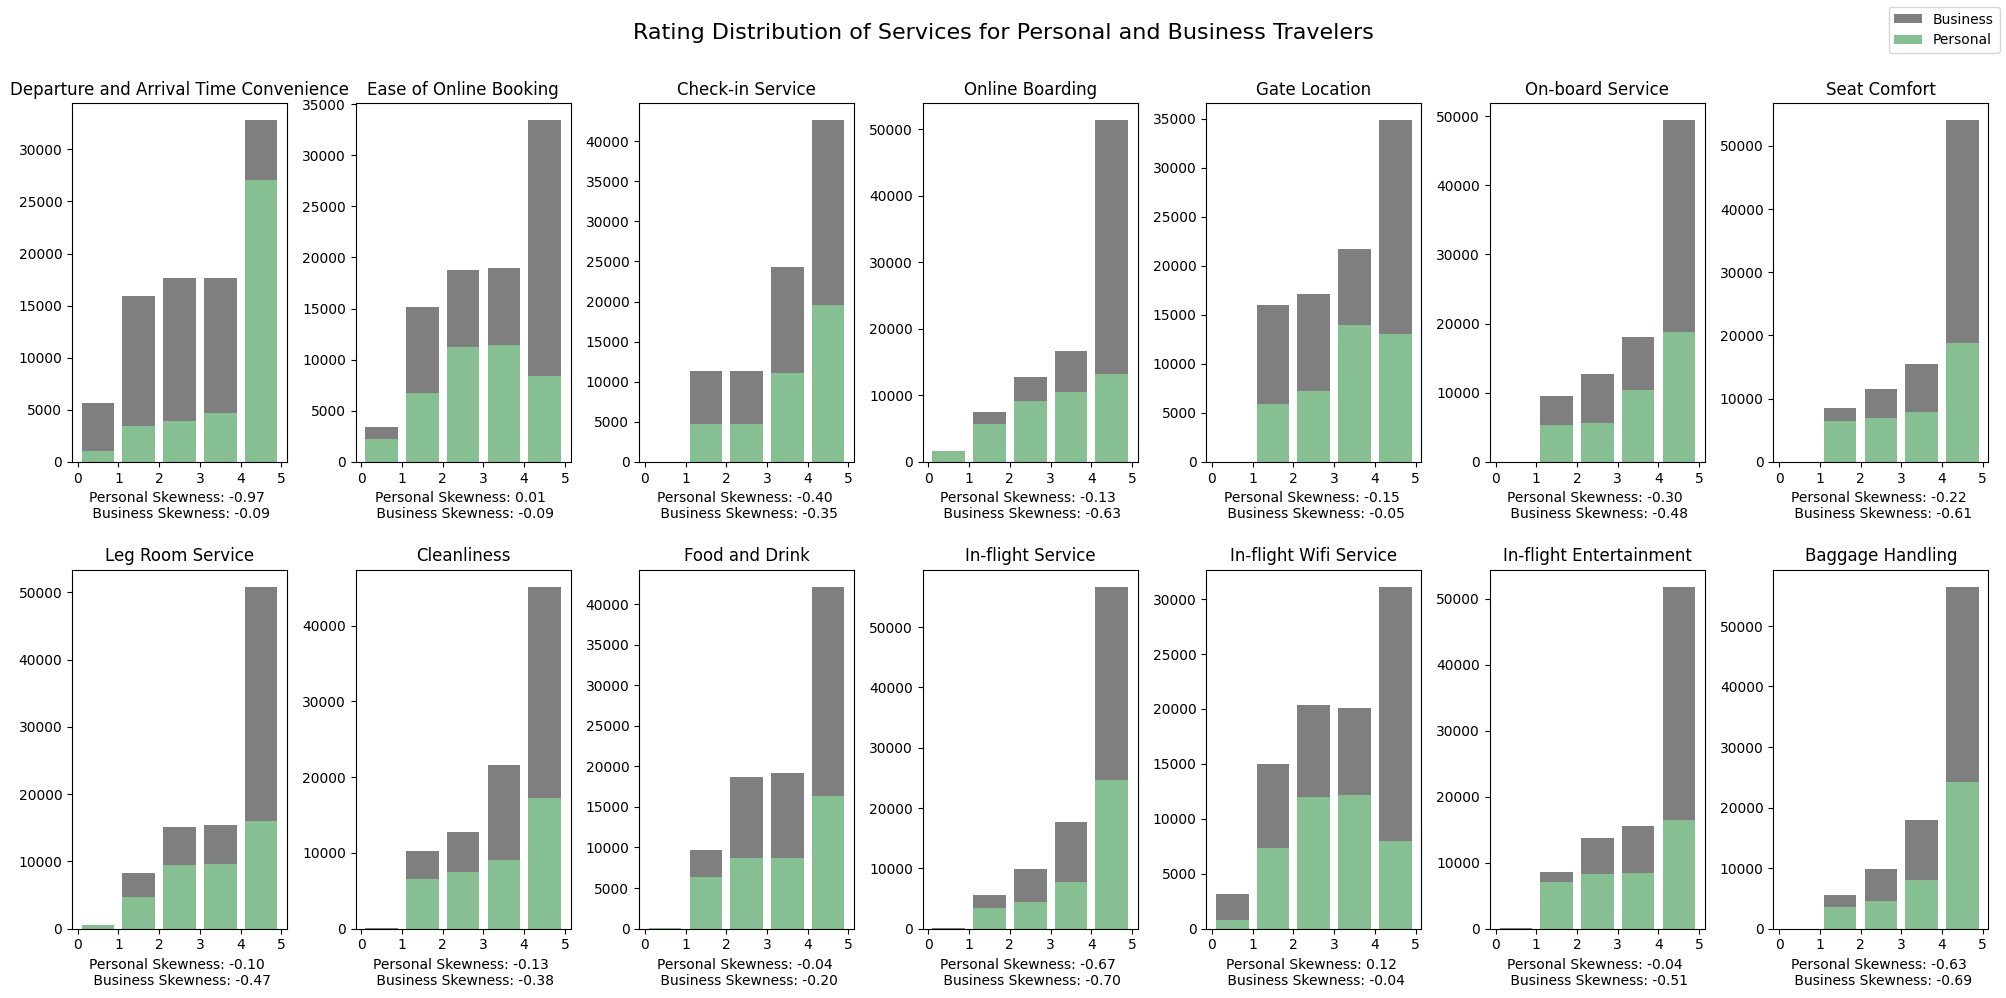
\includegraphics[width=0.9\linewidth]{project_files/project_81_0.png}
\caption{\centering Distribution of service ratings highlighted based on traveler type.}
\end{figure}

The difference in skewness could also be attributed to the disparity in the number of Personal and Business travelers, with Personal travelers comprising 40,187 individuals and Business travelers totaling 89,693. This larger sample size for Business travelers introduces more noise to the data, which shouldn't overshadow the significant difference in overall satisfaction between the two groups. Notably, Business travelers are 48\% more likely to be satisfied than Personal travelers.

\begin{figure}[h]
\centering
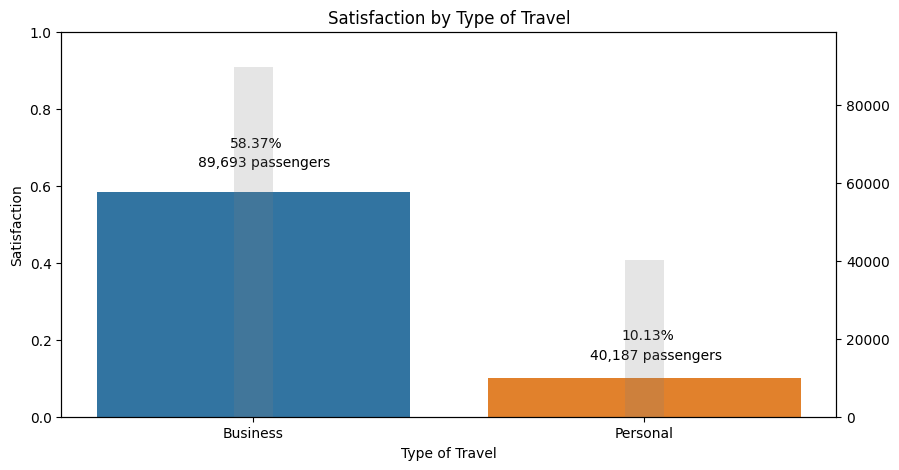
\includegraphics[width=0.6\linewidth]{project_files/project_88_0.png}
\caption{\centering Overall satisfaction of different traveler types along with the number of each type in the sample space.}
\end{figure}

In conclusion, when examining whether there is a meaningful distinction in how different types of passengers rate their overall satisfaction, the data clearly reveals the following: there are over 2.2 times as many Business travelers as Personal travelers, and a substantial 48\% difference exists in their satisfaction levels. This disparity signifies a significant relationship between the type of travel and customer satisfaction. The airline should take these findings into consideration when developing strategies to meet the unique needs and expectations of each passenger group, ultimately fostering higher satisfaction rates and greater customer loyalty.

    \hypertarget{question-7.5}{%
\subsection{Is there a distinct
difference between business class passengers and economy passengers in
terms of their reaction to satisfaction with
food-and-drink?}\label{question-7.5}}

The analysis indicates that there are notable differences in satisfaction levels with food-and-drink between business class passengers and economy passengers (A6). Business class travelers demonstrate a higher mean satisfaction rating in this aspect, with a correlation coefficient of 0.23, while economy passengers exhibit a lower mean satisfaction rating with a correlation coefficient of 0.14. These correlation coefficients are considered negligible, suggesting that there is no strong relationship between food-and-drink satisfaction and overall satisfaction for either group.

\begin{table}[!h]
    \centering
    \begin{tabular}{|c|c|c|}
        \hline
        Class & Food and Drink  &   Satisfaction \\
        \hline
        Business  &      3.329955   &     0.694434 \\
        \hline
        Economy Plus  &      3.110403   &     0.246414 \\
        \hline
        Economy  &      3.086556   &     0.187673 \\
        \hline
    \end{tabular}
    \caption{\centering Pearson correlation coefficient between food and drink service rating and percentage of overall satisfaction across all passenger classes}
    \label{tab:7-4-1}
\end{table}

However, when comparing overall satisfaction among the three passenger classes, a significant variation emerges. The overwhelming majority (69\%) of Business class travelers express satisfaction with their flight experience, whereas only 18\% of Economy passengers report being satisfied with the airline's services. Furthermore, despite having a similar number of passengers, Economy Plus travelers display significantly lower satisfaction levels (45\% difference) compared to Business class passengers, warranting a focus on improving their experience. 

\begin{figure}[h]
\centering
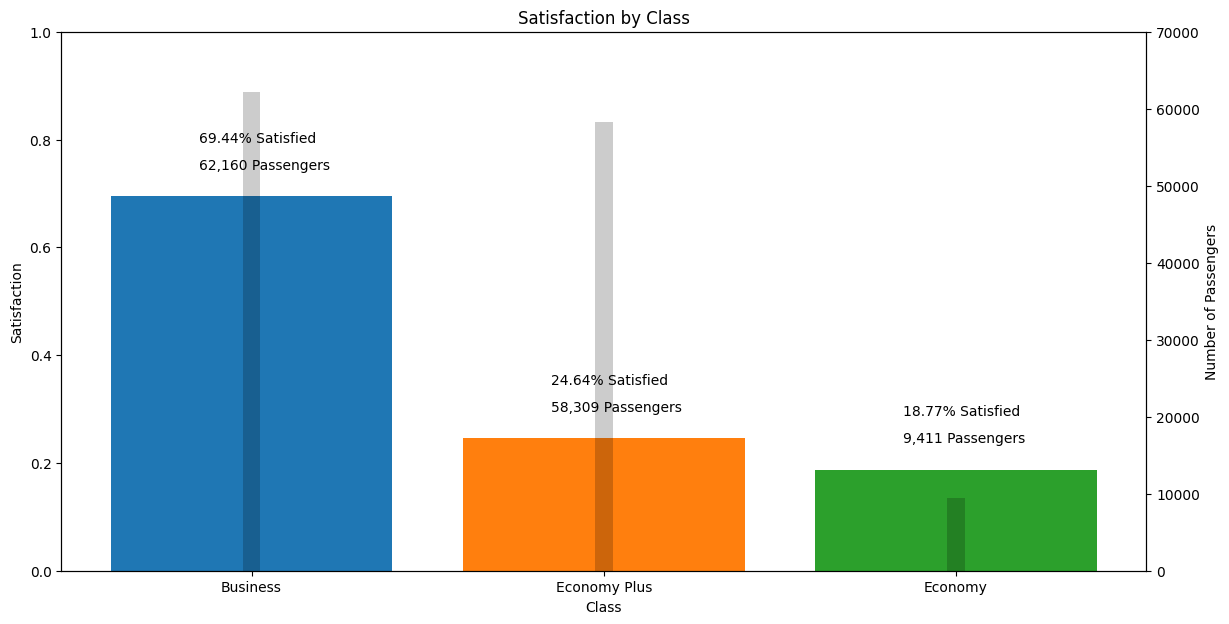
\includegraphics[width=0.6\linewidth]{project_files/project_94_0.png}
\caption{\centering Overall satisfaction percentage of passengers separated by classes.}
\end{figure} 

Analyzing the correlations between overall satisfaction and the food and drink service for each class (Business, Economy, and Economy Plus) yields correlation coefficients of 0.23, 0.14, and 0.26, respectively. These values indicate weak correlations, implying that satisfaction with food and drink does not strongly influence overall satisfaction for any of the classes. However, the Business class exhibits higher correlations with other services, such as Online Boarding and In-flight Entertainment, both having a correlation coefficient of 0.51, indicating that these services play a more significant role in shaping overall satisfaction for Business class passengers. Interestingly, across all classes, the In-flight service demonstrates a notable correlation with overall satisfaction, suggesting that improvements in this area could positively impact passengers' overall satisfaction levels. 

\begin{figure}[h]
\centering
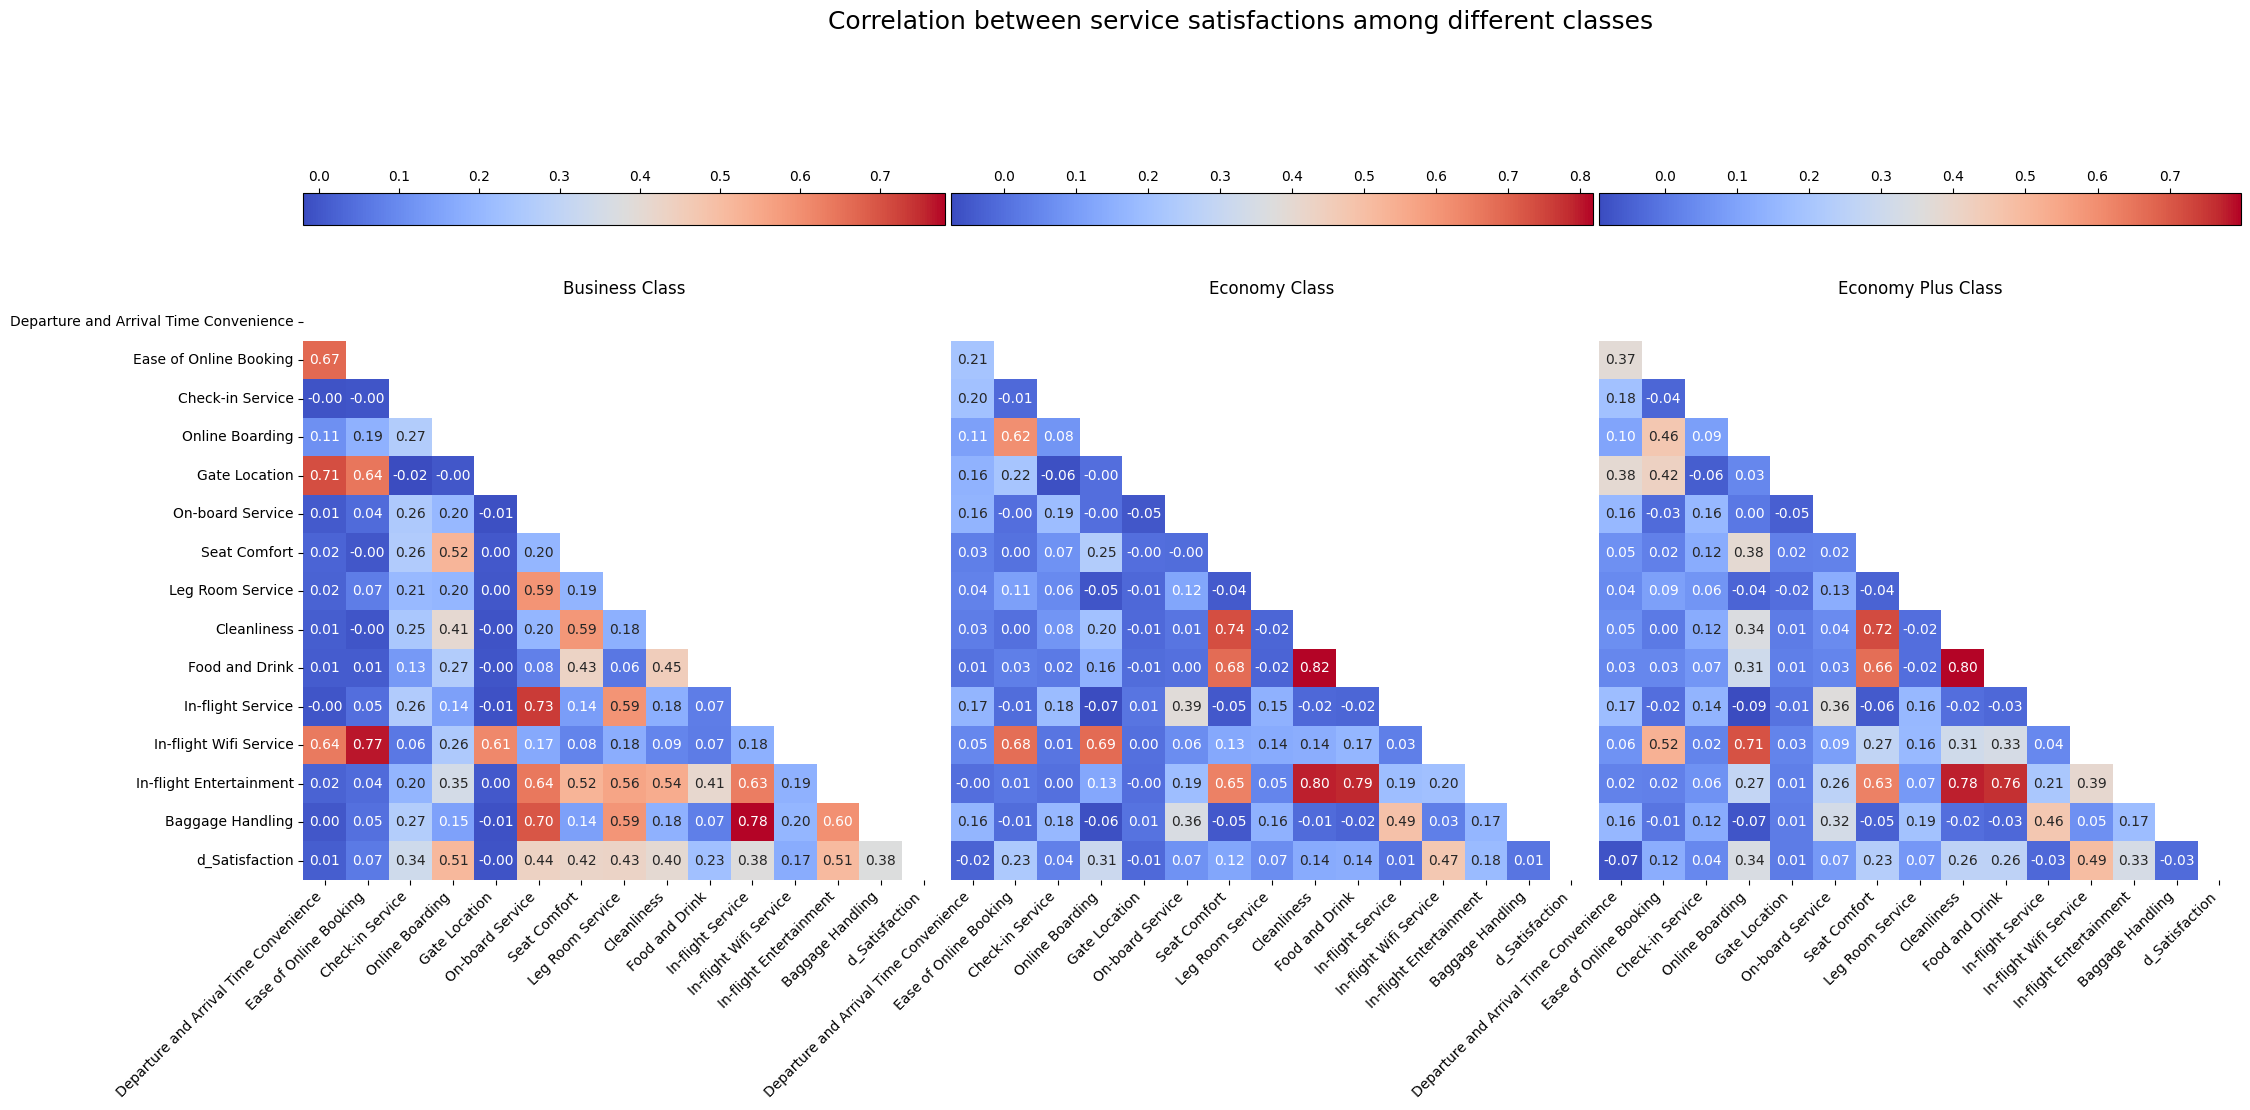
\includegraphics[width=0.9\linewidth]{project_files/project_97_0.png}
\caption{\centering Correlation matrix of pearson coefficients between overall satisfaction rating and each service attribute, seperated by passenger class.}
\end{figure}

In conclusion, while there are differences in satisfaction with food and drink between Business class and Economy passengers, the correlation between this aspect and overall satisfaction is weak for both groups. However, overall satisfaction levels vary significantly among the three classes, with Business class passengers expressing higher satisfaction compared to Economy and Economy Plus passengers. The findings underscore the need to focus on enhancing the experience of Economy Plus passengers to bridge the satisfaction gap with Business class travelers, given the comparable number of passengers in each class. Additionally, attention should be given to improving the In-flight service across all classes, as it emerges as an influential factor affecting overall passenger satisfaction.
    
%     Are the three classes of passengers equally satisfied with
% their
% services? From the above tables we can see observe that there isn't any major
% differences between the classes as their mean values are almost the
% same, as well as the standard deviation. It is, again, noteworthy that
% the Business and Economy classes take up a much larger sample size, yet
% they all keep a relatively equal mean overall satisfaction rating. From the above comparison between airline classes and overall
% satisfaction, we can see that the overwhelming majority (69\%) of
% Business class travelers are satisfied with their flight experience,
% while only 18\% of Economy travelers are satisfied with the services
% offered by the airline.

% Something even more staggering is that there was only 7\% more Business
% class passengers than Economy Plus, yet there was a 45\% difference in
% satisfaction between the two classes. From this, we can conclude that
% the airline should focus on improving the experience of Economy Plus
% passengers, as they are significantly lacking in satisfaction compared
% to the Business class while also making up almost the same amount of
% passengers.

%     The correlation between overall satisfaction and the food and drink
% service for the Business, Economy and the Economy Plus classes is
% \emph{0.23}, \emph{0.14}, and \emph{0.26} respectively. All of which are
% considered to be negligible. Just like in the previous section, the
% business class has a much bigger sample size (62,160) than the economy
% plus class (9411) and the economy class (58,309). The highest
% correlation between overall satisfaction and other services for the
% business class is \emph{0.51} with Online Boarding and In-flight
% Entertainment tied. Something interesting to note is that the In-flight
% service is among the highest of correlations across all classes, meaning
% that single service could be a major influence on the final
% satisfaction rating.


    % Add a bibliography block to the postdoc
    

    \begin{thebibliography}{9}
    \bibitem{authors-gh}
    Dániel Bence Papp - GitHub - Airline Satisfaction repository \\
    \url{https://github.com/chef-danny-d/airline-satisfaction)}

    \bibitem{3d-plot}
    3D scatter plot - MatPlotLib Docs \\
    \url{https://matplotlib.org/stable/gallery/mplot3d/scatter3d.html}
    
    \bibitem{tds}
    Association Rules - Towards Data Science \\
    \url{https://towardsdatascience.com/association-rules-2-aa9a77241654}

    \bibitem{mlext}
    mlxtend Frequency Patterns \\
    \url{https://rasbt.github.io/mlxtend/api_subpackages/mlxtend.frequent_patterns/#apriori}
    
    \bibitem{datacamp}
    Data Camp Association rule mining \\
    \url{https://www.datacamp.com/tutorial/association-rule-mining-python}
    
    \bibitem{medi}
    Association rules with python \\
    \url{https://medium.com/@mervetorkan/association-rules-with-python-9158974e761a}
    
    \bibitem{pandas-docs}
    Pandas Docs \\
    \url{https://pandas.pydata.org/docs/reference/api/pandas.DataFrame.quantile.html}
    
    \bibitem{seaborn-docs}
    Seaborn Docs \\
    \url{https://seaborn.pydata.org/tutorial/color_palettes.html}
    
    \bibitem{gfg}
    GeeksForGeeks Python Pandas \\
    \url{https://www.geeksforgeeks.org/python-pandas-dataframe-corr/#}
    
    \bibitem{}
    Frequency Patterns / Association Rules - User Guide \\
    \url{https://rasbt.github.io/mlxtend/user_guide/frequent_patterns/association_rules/}
    
    \bibitem{}
    Stack Abuse - Association Rule Mining via Apriori Algorithm \\
    \url{https://stackabuse.com/association-rule-mining-via-apriori-algorithm-in-python/}



\end{thebibliography}
\end{document}
